\documentclass[preprint,12pt]{elsarticle}
\usepackage{amssymb}
\usepackage{amsthm}
\usepackage{graphicx}
\usepackage{graphics}
\usepackage{subfigure}
\usepackage{longtable}
\usepackage{float}
\usepackage{amsmath}
\usepackage{gensymb}
\usepackage{booktabs}
\usepackage{caption}
\usepackage [justification=centering] { caption }
\UseRawInputEncoding

\journal{Journal of energy storage}
\begin{document}
	\captionsetup[figure]{labelfont={bf},name={Fig.},labelsep=period} 
	\captionsetup[table]{labelfont={bf},labelformat={default},labelsep=period,name={Table}}
\begin{frontmatter}
	
	\title{Thermal energy storage system based on nanoparticle distribution optimisation for enhanced heat transfer}
		\author[a]{Bichen Shang} 
			\author[a]{Liwei Zhang} 	
	\author[a]{Bingbing Li} 
	\author[a]{Yutao Huo\corref{cor1}}
	\affiliation[a]{organization={School of Low-Carbon Energy and Power Engineering, China University of Mining and Technology},
		city={Xuzhou},
		postcode={221116},             
		country={China}}
	
\begin{abstract}
	
As a new type of heat transport medium with high efficiency and high heat transfer performance, nanofluids can effectively improve the heat transfer performance of thermal systems. In this paper, a lattice Boltzmann method is employed to propose a novel thermal storage system with optimised nanoparticle distribution using spacer-separated nano-enhanced PCM with spacer arrangement. The thermal energy storage units are separated by thermal insulation and heated by means of thermally conductive fluid channels. The effects of Rayleigh number, volume fraction and layout pattern are investigated. It is shown that the larger the Rayleigh number is, the more intense the reaction of the heat storage system is; it is concluded that the strong convection phenomenon in the upper left side region is more than that in the lower left side, and the volume fraction in the lower left side can be reduced to enhance the efficiency of this heat transfer in order to achieve a faster melting rate. The various distributions studied in this paper all have the effect of accelerating the melting rate to varying degrees compared to Type 1. The present study shows that increasing the volume fraction of phase change material in the upper left side of the square cavity has a promoting effect on the melting rate when compared to the lower side, and the larger the difference between the two, the better the effect is.

	\end{abstract}
	
	\begin{graphicalabstract}
		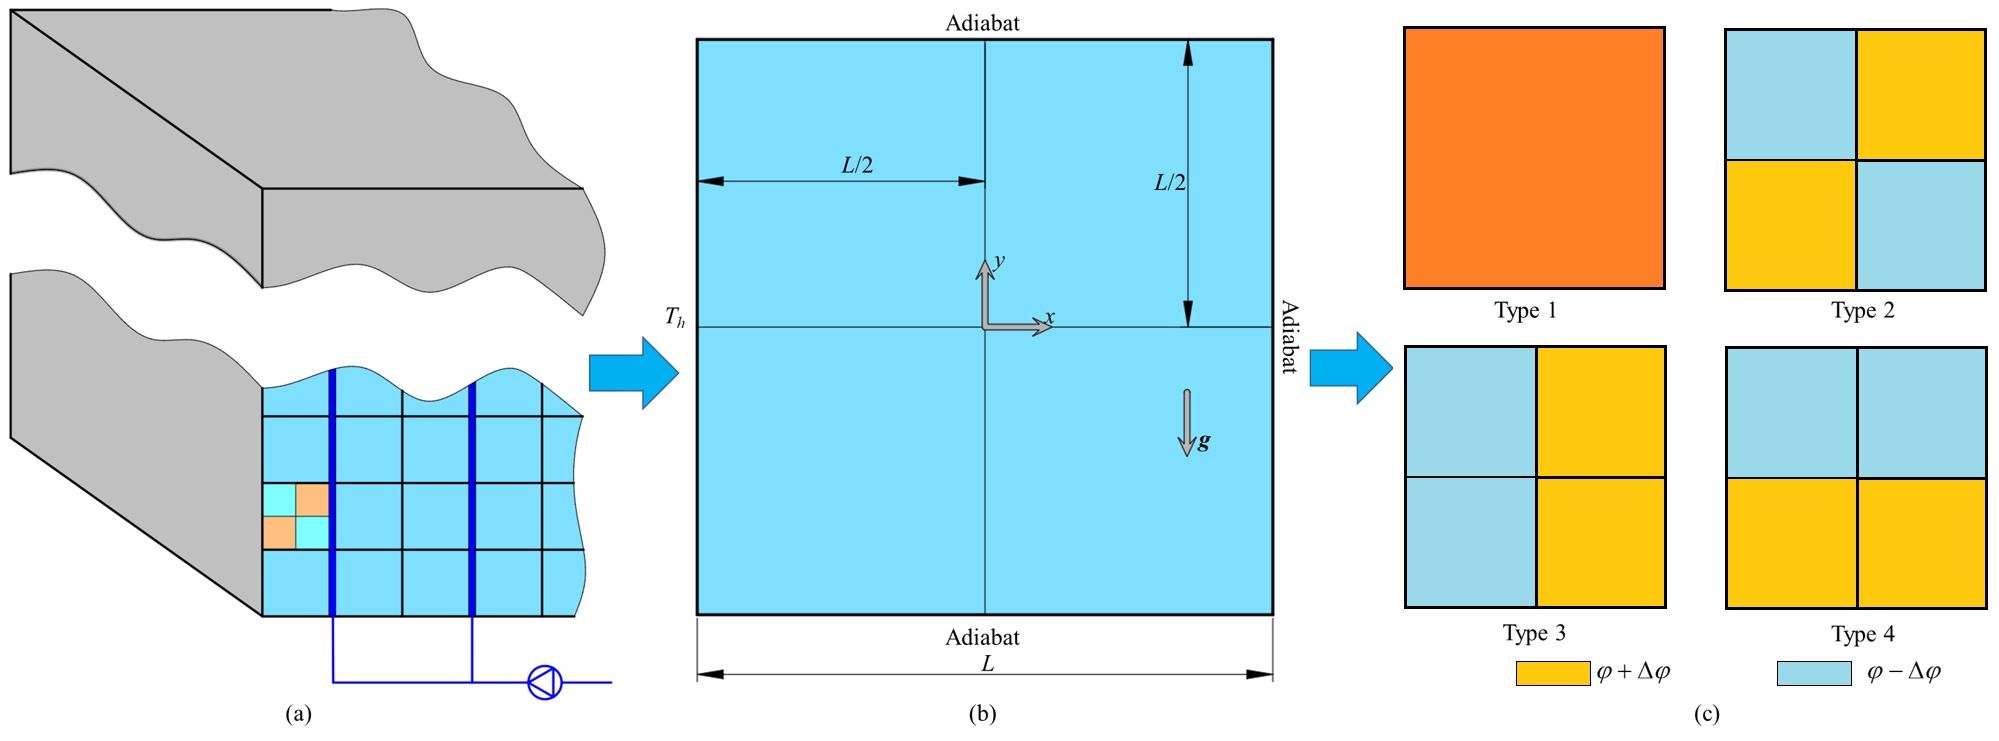
\includegraphics[scale=0.5]{Fig/Numerical_Model.png}
	\end{graphicalabstract}
	
	\begin{highlights}
		\item Thermal energy storage units are separated by thermal insulation and heated by means of thermally conductive fluid channels.
		\item A variety of distributions in this paper have the effect of enhancing heat transfer, where the distribution under type 2 has a faster melting rate, which is increased by 2.13\%, 1.84\%, 1.9\%, 1.72\%, 1.8\%, 1.89\% at Rayleigh number change from $ 5\times10^3 $ to $ 10^6 $, compared to type 1.
		\item Optimising nanoparticle volume fraction in distributed energy storage systems.
	\end{highlights}
	
	\begin{keyword}
		Thermal energy storage, Seperate plate, Lattice Boltzmann, Nano-enhanced PCM

	\end{keyword}
	
\end{frontmatter}
\section{Introduction}
Thermal energy storage (TES) is one of the important technology to improve the usage of new energy, such as solar energy, wind energy and geothermal energy \cite{XIAO2023107066}. Besides, by applying the TES, the waste heat of chemical industry can be recovered as well\cite{RN1214}. Thermal conductivity is the most important evaluation index of TES, and the thermal conductivity of Phase Change Material(PCM) is one of the important factors affecting\cite{Prieto2019ThermalES}. Consequently, in order to improve the effectness of TES, several enhanced methods are proposed.

It is widely noted that most of the PCM possesses low thermal conductivity and the effective way to improve heat transfer rate of TES is to enlarge the thermal conductivity, such as inserting the high-thermal-conductivity material into PCM. Feng et al. \cite{RN1215} used the copper foam to enhance the heat transfer rate of paraffin. They studied the effective protection time of PCM heat sink and found that when the filling ratio of copper foam was increased from 0 to 40\%, the melting fraction of paraffin was increased from 20.3\% to 43.3\%. Fan et al. \cite{RN1218} proposed that using carbon foam was able to improve the photo-thermal conversion capability and the results showed that with carbon foam, the charging and discharging efficiency was nearly 90\%. The nickel foam was adopted in TES by Chen et al. \cite{RN1219}. They proposed the fin-foam structure and investigated the solidification process. Furthermore, the fin-foam structure was studied by Du et al. \cite{RN1223} using the 3D numerical model, as well. The complete melting time of the fin-foam structure was reduced by 83.68\% compared with the pure PCM, while the temperature uniformity was increased by 91.12\%. Moveover, the magnetic field was inserted to PCM/copper foam to enhance the natural convection by He et al. \cite{RN1220}. The positive magnetic field accelerated the melting and energy storage rate of PCM/copper foam by 18.2\% and 23.1\%. However, during the solidification process, the effect of magnetic field was weak.
Liao et al. \cite{Liao2018ANE} encapsulated phase change materials into a thermal energy storage system and applied it to the utilization of solar energy. A linear regression method is proposed as a new effective thermal conductivity correlation by using simulation results that incorporate a natural convection model.
Jinming et al. \cite{Shi2020TuningTF} showed that when the weight of carbon nanotubes is only 5\%, the thermal conductivity of polyurethane-carbon nanotubes composites increased by 2.3 times, and the efficiency of solar thermal energy storage reached 85.89\%, which contributes to the subsequent further exploration of composite PCMs for solar energy applications.

Another effective way to enhance the thermal performance of TES is to inserting the high-conductivity fin. Oztop et al. \cite{RN1224} used artificial neural network to design the structure of fin applying in phase change TES. They found that the fin could enhance the heat transfer significantly. In H-shaped TES system, the effects of fin angle on the melting process were investigated by Izadi et al. \cite{RN1231}. They found the heat transfer enhancement was resulted from the conducitive heat transfer in the fin. Mostafavi and Jain \cite{RN1225} presented theoretical analysis of heat transfer between base wall and PCM using fin. The improved system was applied to thermal management. The fin based heat sink was adopted in high power electronics cooling as well \cite{RN1232}. Furthermore, the ladder-shaped fin was proposed by Liu et al. \cite{RN1227} in waste heat recovery. The TES device was tested numerically and the melting time could be reduced by 52.2\% compared to the original straight fin case. Guo et al. \cite{RN1226} demonstrated that in the complete melting time was decreased by 69.59\% by using non-uniform angled fins in TES. Two types of fins, the punched one and slit one, inside a shell-and-tude heat exchanger were studied by Ding and Liu \cite{RN1230}, numerically. The results showed that the improvement of heat transfer was derived from decrease of the blockage effect.

Existing research teams are investigating thermal storage systems by synthesizing and improving the thermal properties and stability of eutectic salts to optimize the structure of thermal storage devices. Chlorides, fluorides, and carbonates are potentially promising thermal storage media for use as potential thermal storage media in high temperature thermal storage systems\cite{Wang2023ARO}. The researchers have determined and calculated the melting point, thermal conductivity, latent heat, and other parameters of these three eutectic salts\cite{Wang2023ComprehensivePO,Wu2023ThermodynamicCA}, which provide important guidance for thermal storage materials for concentrating solar power plants. And enhanced heat transfer through CuO\cite{Wu2023ComprehensiveTP}.

It is noted that traditional heat transfer media such as water, glycol, heat transfer oil, etc., but the thermal conductivity is low. Since the 1990s, with the development of nanotechnology, researchers began to explore the application of nanomaterials technology in the field of enhanced heat transfer, and to study a new generation of high-efficiency heat transfer and cooling technology. In 1995, Professor S.U.S. Choi of the Aragon National Laboratory of the United States for the first time put forward the concept of "nanofluid" \cite{1995Developments}, the innovative combination of nanotechnology and the traditional field of thermal engineering has a very broad application prospect and potentially significant economic value. Nanotechnology and thermal engineering as a traditional field innovatively combined with a very broad application prospects and potentially significant economic value. As a new type of heat transport medium with high efficiency and high heat transfer performance, nanofluids can effectively improve the heat transfer performance of thermal systems, and improve the performance indexes of thermal systems, such as high efficiency and low resistance compactness.Over the past two decades, the Lattice Boltzmann Method (LBM) as an efficient and powerful method for fluid mechanics and heat transfer problems.The LBM can be used to simulate flows at the micro- and nanoscale and is well suited for parallel computing or GPU acceleration\cite{Chen2018MultiGPUST}.

According to the existing papers, the previous studies did not consider the effect of separating the NEPCM by the spacer with the arrangement. In this paper, a new thermal storage system for optimally distributing nanoparticles has been proposed. The effects of Rayleigh number, volume fraction and layout mode are investigated by LBM. The results are beneficial to the design of TES system. 

\section{Model description}
\subsection{Pysical model}
The schematic of TES tank is shown in Fig.\ref{Fig_Numerical_Model} (a). Each TES unit is divided by the insulation material and heated by the channel with heat trasnfer fluid, driven by the pump. During energy storge process, the heat carried by the heat transfer fluid is transfrred to PCM. For convenience, one of the TES unit ($L\times L$) is investigated, as shown in Fig.\ref{Fig_Numerical_Model} (b). The effects of arrangement of NEPCM are studied and schematic is shown in Fig.\ref{Fig_Numerical_Model} (c). Four kinds of arragements are considered. In Type 2-4, each part divided by seperate plate is filled with NEPCM. 
Within each of the type, regions are named in order from left to right, top to bottom as ``0" or ``1". For example, the type 2 respected the distribution of ``0101".

It is noted that thermal properties of NEPCM depend on volume fraction of nanoparticle. In this paper, the Al$_2$O$_3$ nanoparticle is applied and the volume fraction is $\varphi$. To ensure the total latent heat in the unit, the NEPCM with $+$ and $-$ is filled in parts of ``1" and ``0", respectively.

\begin{figure}[H] 
	\centering
	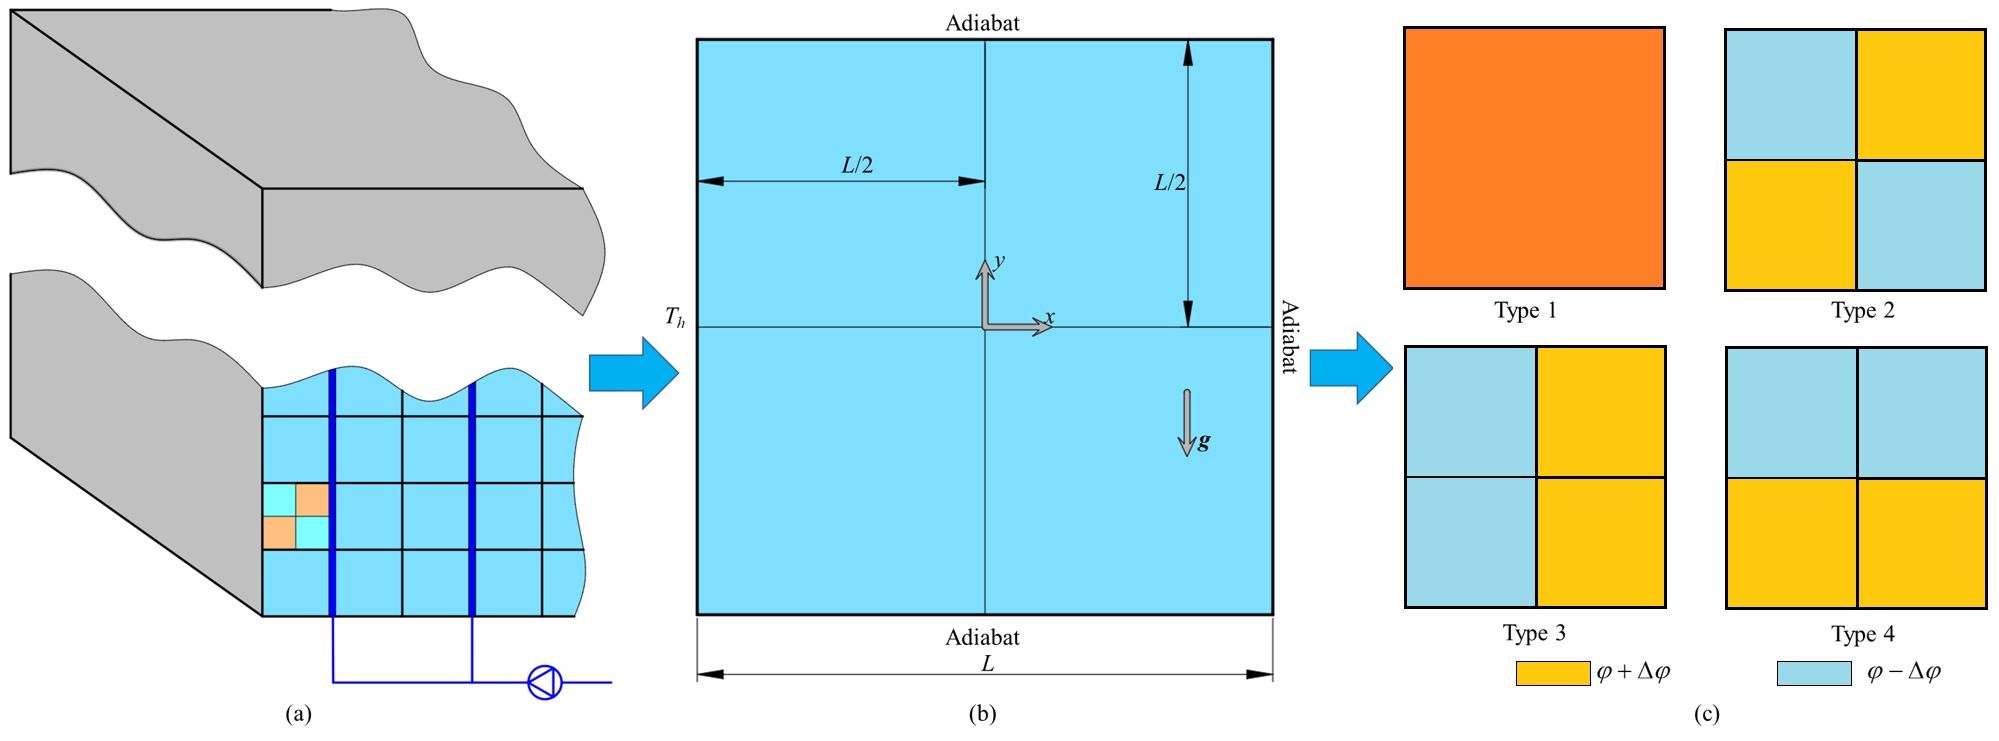
\includegraphics[scale=0.4]{Fig/Numerical_Model.png}

	\caption{The schematics of (a) thermal energy storage tank, (b) thermal energy storage unit and (c) arrangement of NEPCM } 
	\label{Fig_Numerical_Model}
\end{figure}

\subsection{Boundary conditions}
The channel is simplified as a boundary with constant temperature $T_h$. Other boundaries are set as adiabatic. Two seperate plates are placed at $x=L/2$ and $y=L/2$. The thickness of seperate plate is nearly 0 and the material of seperate plate is NEPCM as well.The NEPCM is solid and the initial temperature is $T_0$.

\subsection{Numerical model and Governing equations}

In this study, the NEPCM is assumed as Newtonian fluid and flow is incompressible. The enthalpy-transforming LBM is applied to reveal the flow and heat trasnfer behavior. The evolution equations of density and enthalpy distribution functions are listed as follows \cite{RN25,RN847}:

\begin{equation}
	f_i(x+e_i\Delta t,t+\Delta t)=f_i(x,t)-\frac{1}{\tau_f}[f_i(x,t)-f_i^{eq}(x,t)]+\Delta t F_i
	\label{Evolutions_of_Density}
\end{equation}
\begin{equation}
	g_i(x+e_i\Delta t,t+\Delta t)=g_i(x,t)-\frac{1}{\tau_g}[g_i(x,t)-g_i^{eq}(x,t)]
	\label{Evolutions_of_Enthalpy}
\end{equation}
where $f_i$ and $g_i$ are density and enthalpy distribution functions in direction $i$. $f_i^{eq}$ and $g_i^{eq}$ are the equilibrium distribution functions, as follows \cite{RN570}:
\begin{equation}
	f_i^{eq}=\omega_i\rho_{bulk}
	\left[
	1+\frac{e_i\cdot u}{c_s^2}+
	\frac{{
			\left(e_i\cdot u\right)
		}^2}{2c_s^4}
	-\frac{u^2}{2c_s^2}
	\right]
	\label{f_eq}
\end{equation}
\begin{equation}
	g_i^{eq}=\omega_i
	\left[
	H+C_{p,bulk}T
	\left(
	\frac{e_i\cdot u}{c_s^2}+\frac{
		\left(e_i\cdot u\right)			
		^2}{2c_s^4}
	-\frac{u^2}{2c_s^2}
	\right)
	\right]
	+\varpi_i(C_{p,bulk}T-H)
	\label{g_eq}
\end{equation}
where $\omega_i$ and $e_i$ are the weighting coefficient and discrete velocity in direction $i$. $c_s$ is the lattice sound speed. In this paper, the D2Q9 collision model is adopted, as follows:
\begin{equation}
	\omega_i=
	\left\{
	\begin{aligned}
		\frac{4}{9}\qquad &i=0 \\
		\frac{1}{9}\qquad &i=1\sim4 \\
		\frac{1}{36}\qquad&i=5\sim8
	\end{aligned}
	\label{omega_i}
	\right.
\end{equation}
\begin{equation}
	{e_i} = \left\{ 
	\begin{aligned}
		\left( {0,0} \right)\;\;\;\;\;\;\;\;\;\;\;\;\;\;\;\;\;\;\;\;\;\;\;\;\;\;\;\;\;\;\;\;\;\;\;\;\;\;\;\;\;\;\;\;\;\;\;\;\;\;i = 0 \hfill \\
		c\left( {\cos \left[ {\frac{\pi }{2}\left( {i - 1} \right)} \right],\sin \left[ {\frac{\pi }{2}\left( {i - 1} \right)} \right]} \right)\;\;\;\;\;\;\;\;\;\;\;\;i = 1,2,3,4 \hfill \\
		\sqrt 2 c\left( {\cos \left[ {\frac{\pi }{4}\left( {2i - 1} \right)} \right],\sin \left[ {\frac{\pi }{4}\left( {2i - 1} \right)} \right]} \right)\;\;\;\;i = 5,6,7,8 \hfill \\ 
	\end{aligned} 
	\right.
\end{equation}
where $c=\Delta x/\Delta t$ is the lattice speed. $\varpi_i$ in Eq. (\ref{g_eq}) is the extra weight coefficient, as follows:
\begin{equation}
	{\varpi _i} = \left\{ \begin{gathered}
		- \sum\limits_{i = 1}^8 {{\omega _i}} \;\;\;\;\;\;\;\;i = 0 \hfill \\
		{\omega _i}\;\;\;\;\;\;\;\;\;\;\;\;\;\;i \ne 0 \hfill \\ 
	\end{gathered}  \right.
\end{equation}

In Eq. (\Ref{Evolutions_of_Density}), $F_i$ in the right hand side is the discrete body force term in direction $i$, obtained by:
\begin{equation}
	{F_i} = {\omega _i}\left( {1 - \frac{1}{{2{\tau _f}}}} \right)\left( {\frac{{{e_i} - u}}{{c_s^2}} + \frac{{{e_i} \cdot u}}{{c_s^4}}{e_i}} \right) \cdot {\rho}{f_m}
\end{equation}
where $f_m$ is the body force, buoyancy in this paper, computed from:
\begin{equation}
	f_m=g\beta_{bulk} \left(T-T_0\right)
\end{equation}
where $g$ and $\beta$ is the acceleration of gravity (shown in Figure \ref{Fig_Numerical_Model}) and thermal expansion, respectively.

$\tau_f$ and $\tau_f$ in Eq. (\ref{Evolutions_of_Density}) are the dimensionless relaxation times, computed from:
\begin{equation}
	\nu_{bulk} = \frac{\mu_{bulk}}{\rho_{bulk}} = \left( {{\tau _f} - \frac{1}{2}} \right)\Delta tc_s^2
\end{equation}
\begin{equation}
	\alpha_{bulk} =\frac{\lambda_{bulk}}{\rho_{bulk} C_{p,bulk}} = \left( {{\tau _g} - \frac{1}{2}} \right)\Delta tc_s^2
\end{equation}
where $\nu$ and $\alpha$ are the vicosity and thermal diffusivity. After solving Eq. (\ref{Evolutions_of_Density}) and (\ref{Evolutions_of_Enthalpy}), the density, velocity and enthalpy can be computed from the distribution functions, as follows:
\begin{equation}
	\rho  = \sum\limits_i {{f_i}} 
\end{equation}
\begin{equation}
	{\rho}u = \sum\limits_i {{e_i}{f_i}}  + \frac{{\Delta t}}{2}{\rho}{f_m}
\end{equation}
\begin{equation}
	H = \sum\limits_i {{g_i}} 
\end{equation}

In this paper, the Rayleigh number ($Ra$), Prandtl number ($Pr$) and Stefan number ($Ste$) are defined as follows:
\begin{equation}
	Ra = \frac{{g\beta_{PCM} \left( {T_h - {T_0}} \right){L^3}}}{{\nu_{PCM} \alpha_{PCM} }}
\end{equation}
\begin{equation}
	Pr=\frac{\nu_{PCM}}{\alpha_{PCM}}
\end{equation}
\begin{equation}
	Ste=\frac{C_{p,PCM}(T_h-T_0)}{h_{sl}}
\end{equation}
where the subscript $ “PCM” $ denotes pure PCM while the subscript “$bulk$” in above equations denotes NEPCM. Furthermore, the thermal properties of NEPCM is computed from volume fraction, as follows\cite{RN1173,RN1065,RN1174}:
\begin{equation}
	{\rho _{bulk}} = \left( {1 - \varphi } \right){\rho _{PCM}} + \varphi {\rho _{nano}}
\end{equation}
\begin{equation}
	{\left( {\rho {C_p}} \right)_{bulk}} = \left( {1 - \varphi } \right){\left( {\rho {C_p}} \right)_{PCM}} + \varphi {\left( {\rho {C_p}} \right)_{nano}}
\end{equation}
\begin{equation}
	{\lambda _{bulk}} = \frac
	{\lambda _{nano} + 2\lambda _{PCM} + 2\left( \lambda _{nano}- \lambda _{PCM} \right)\varphi }
	{\lambda _{nano} + 2\lambda _{PCM} - 2\left( \lambda _{nano} - \lambda _{PCM} \right)\varphi }
	\lambda _{PCM}
\end{equation}
\begin{equation}
	{\mu _{bulk}} = 0.983{\mu _{PCM}}\exp \left( {12.959\varphi } \right)
\end{equation}
\begin{equation}
	{\left( {\rho \beta } \right)_{bulk}} = \left( {1 - \varphi } \right){\left( {\rho \beta } \right)_{PCM}}
\end{equation}
\begin{equation}
	{\left( {\rho h_{sl} } \right)_{bulk}} = \left( {1 - \varphi } \right){\left( {\rho h_{sl} } \right)_{PCM}}
\end{equation}
	    
	The thermal properties of the ``nanoparticle" and ``PCM" are listed in Table \ref{Thermal_Properties}. According to the thermal properties, the Prandtl number is kept as $Pr=7.0$ in this paper.
	
	\begin{table}[H]
		\centering
		\footnotesize
		\caption{Thermal properties of nanoparticle and PCM}
		\begin{tabular}{cccccc}
			\toprule
			& $\rho$(kg·m$^{-3}$) & $C_p$(J·kg$^{-1}$·K$^{-1}$) & $\lambda$(W·m$^{-1}$·K$^{-1}$) & $\mu$(kg·m$^{-1}$·s$^{-1}$) & $h_{sl}$(J·kg$^{-1}$) \\
			\midrule
			Nanoparticle & 3880 & 765  & 25   & -      & - \\
			PCM          & 930  & 1600 & 0.21 & 9.2$\times10^{-4}$ & 195000 \\
			\bottomrule
		\end{tabular}
		\label{Thermal_Properties}		
	\end{table}
	
\subsection{Model validation}	
Grid independence analysis was performed for this study. The red dashed line in the Fig.\ref{yz} shows the variation of the mean Nusselt number for a grid size of 400$ \times $400 with an error within 3\%. It can be seen that the grid size of 100$ \times $100 and 200$ \times $200 are within this range. Considering the accuracy of the simulation and the rationalization of the use of computational resources, a grid size of 100$ \times $100 is chosen for the calculation.
	\begin{figure}[H]
	\centering
	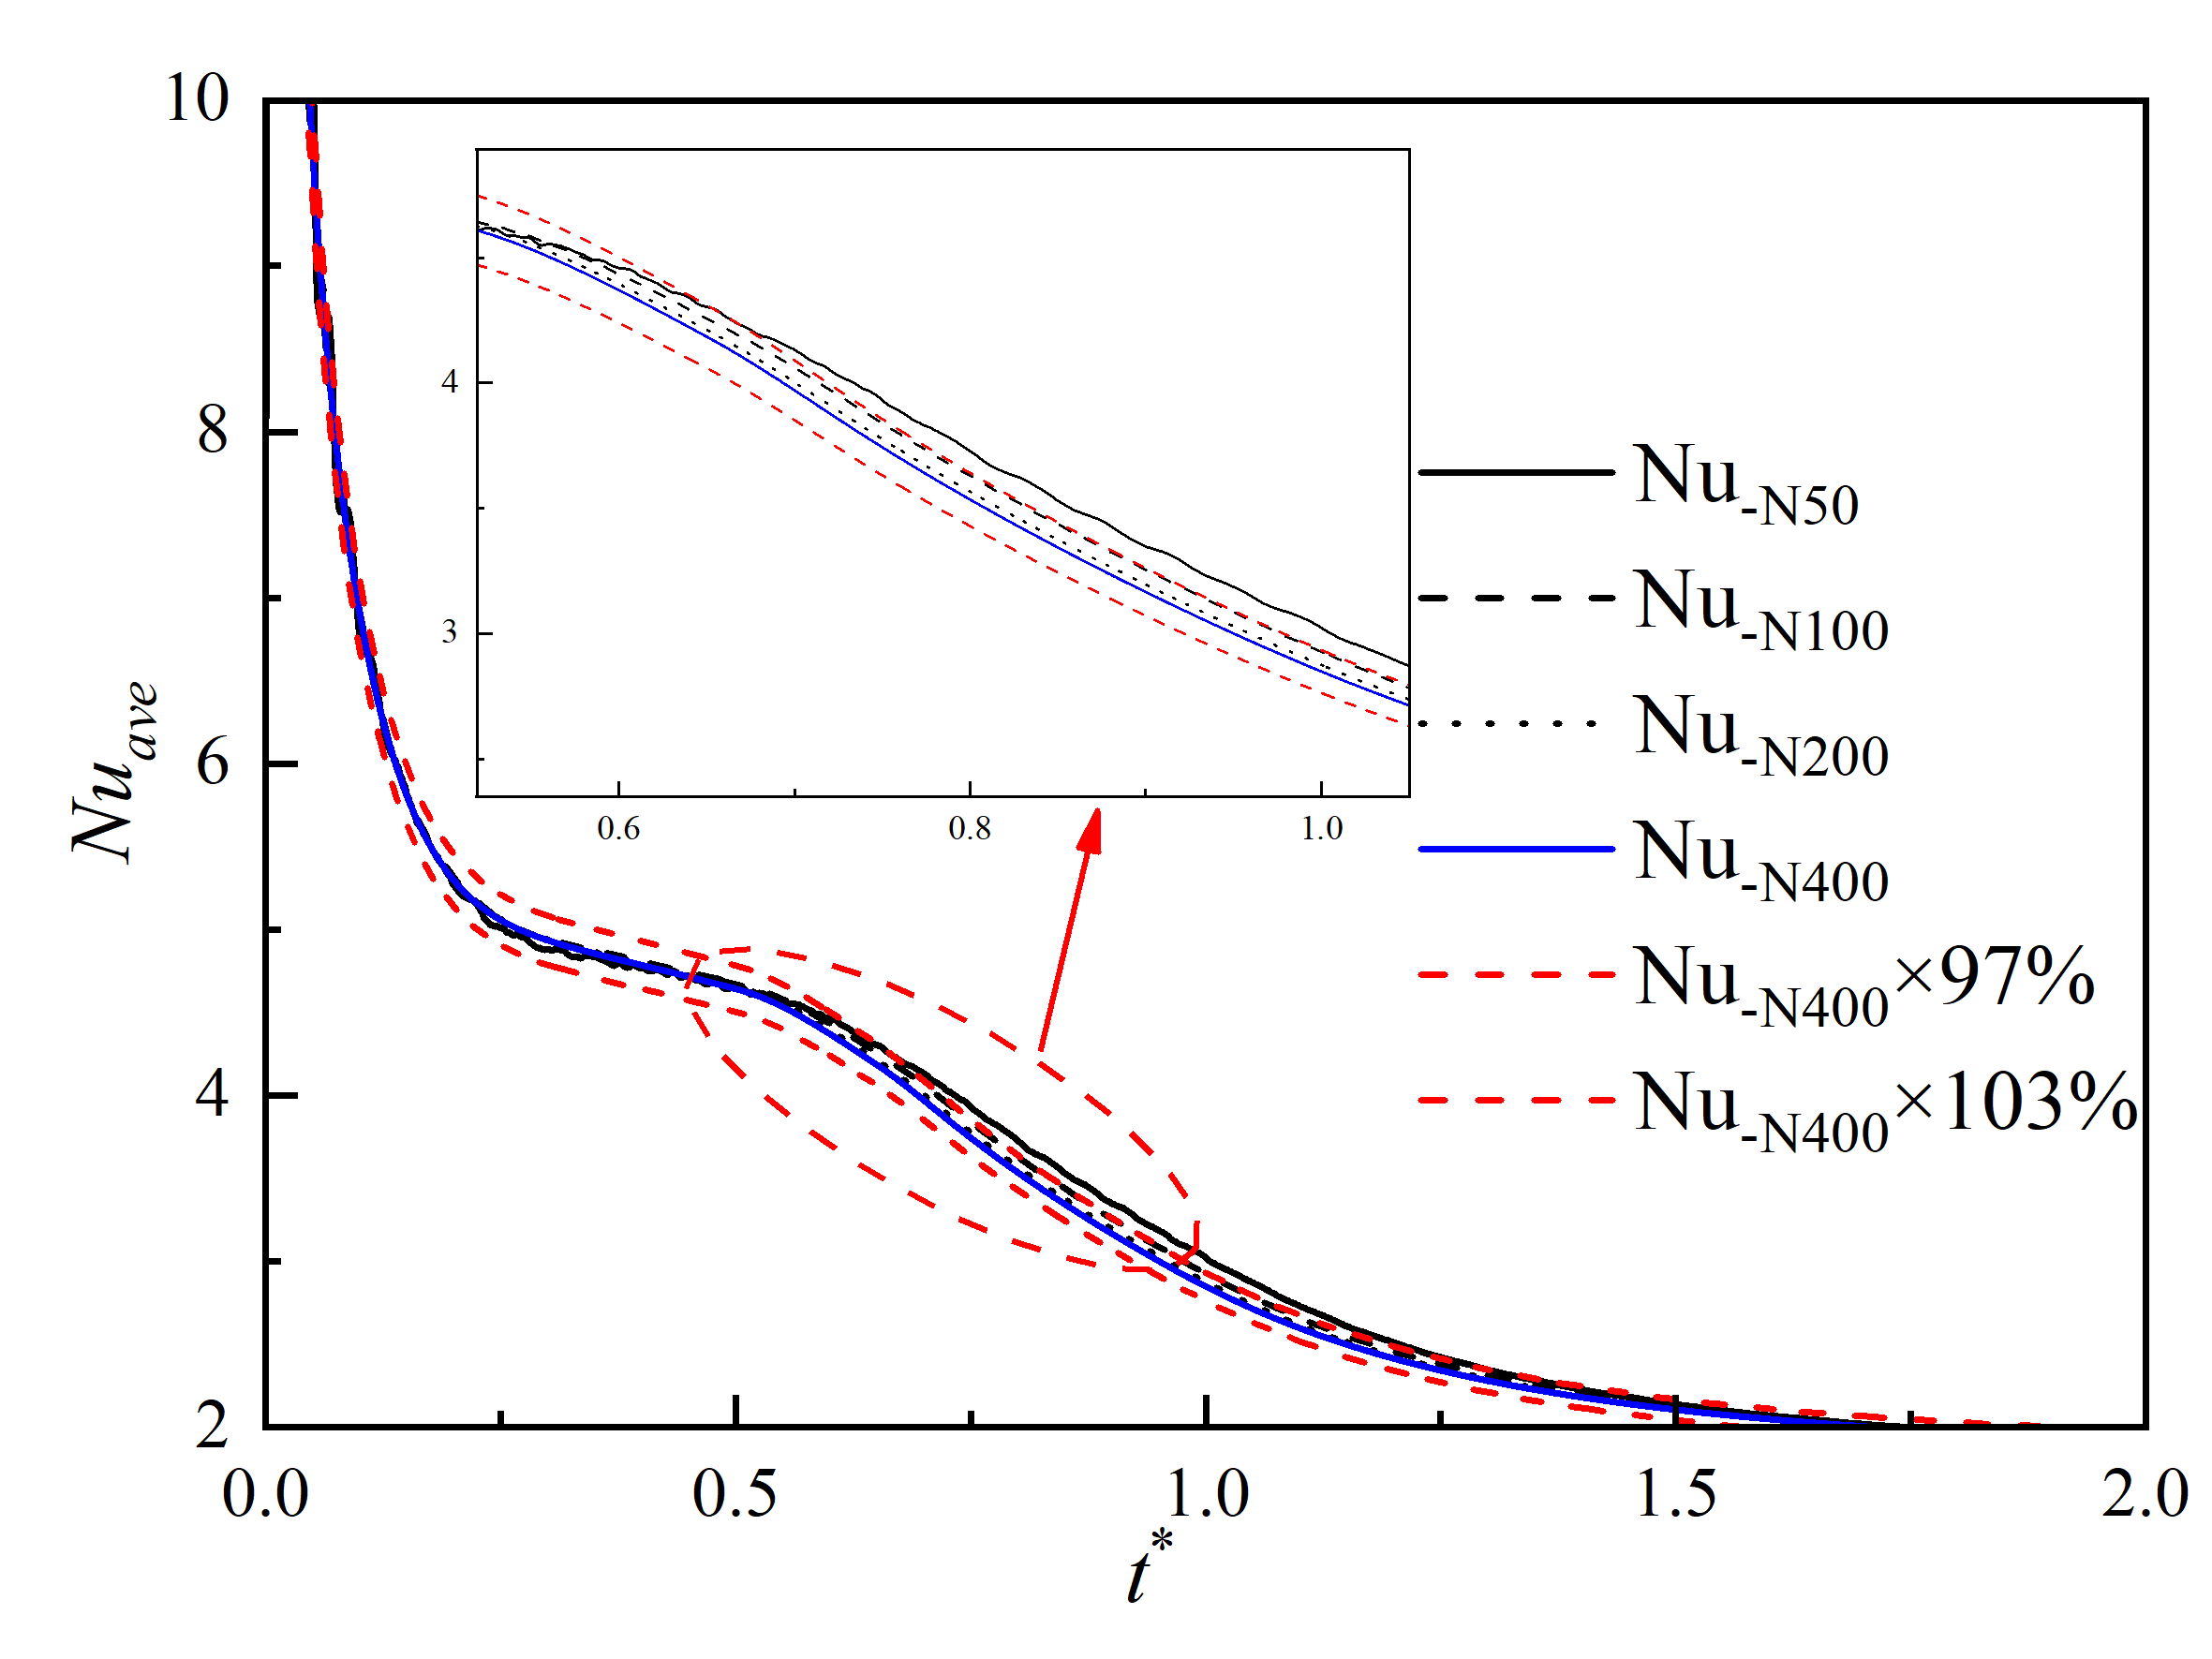
\includegraphics[scale=0.4]{Fig/网格.png}
	\caption{Grid Independence Verification} 
	\label{yz} 
\end{figure}
We applied the LBM to solve the one-dimensional pure thermal conductivity problem and compared the simulated results with analytical solutions shown as Fig.3. The errors between the results obtained by both approaches were1.9\%, 1.3\% and 1\% when \textit{t*}=4, \textit{t*}=10, \textit{t}*=20, respectively. Additionally, we verified the natural convection problem by comparing our model with Mencinger's work\cite{Mencinger2004NumericalSO}. Both the average Nusselt number and the liquid fraction data were presented in Fig.\ref{Fig_yz}, and the results showed excellent agreement. 
The LBM we proposed exhibited errors of less than 2\% compared to Mencinger's work, demonstrating its high reliability.

	\begin{figure}[H]
	\centering
	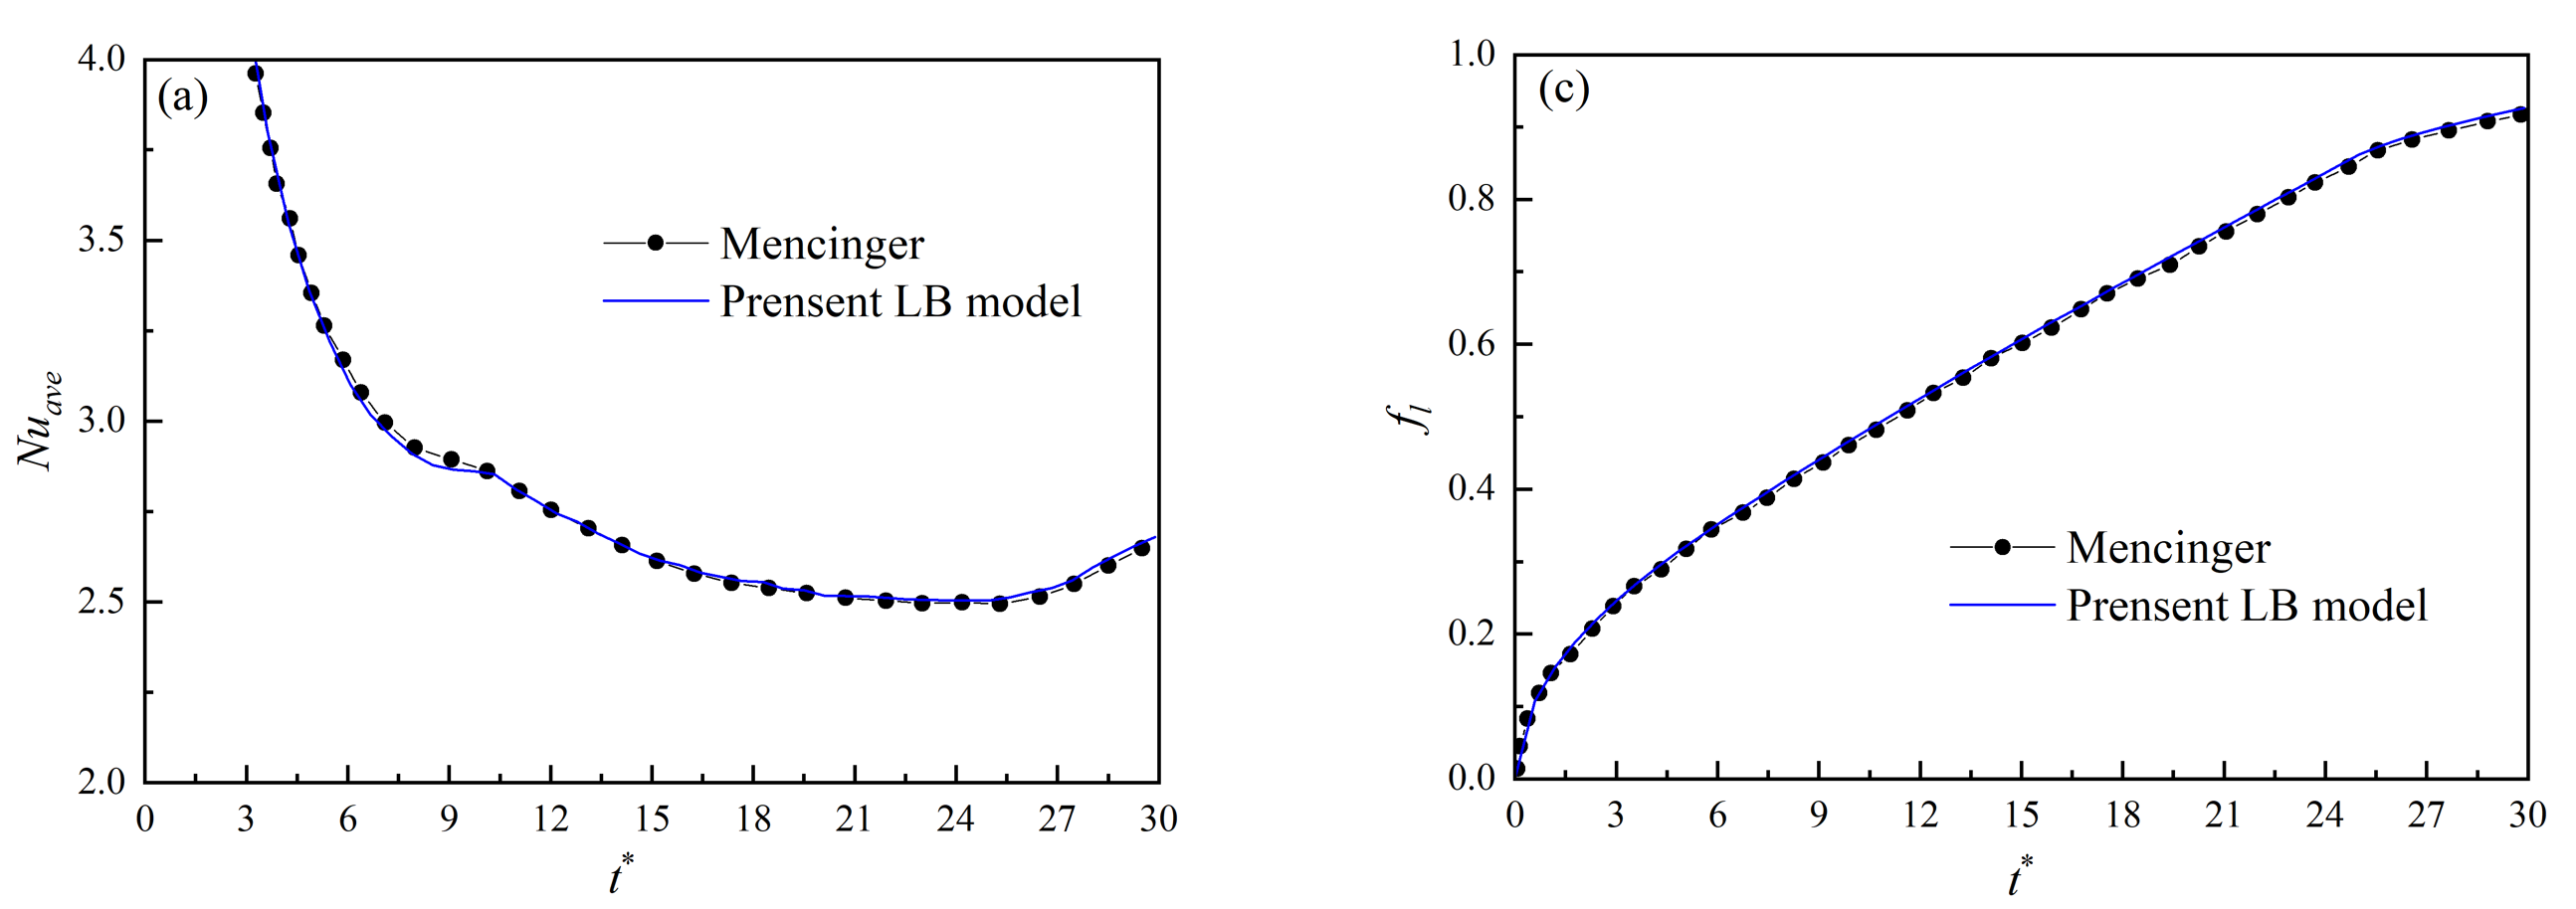
\includegraphics[scale=0.6]{Fig/yanz.png}
	\caption{The variations of (a) average Nusselt number and (b) total liquid fraction with Ra=$ 2.5 \times 10^4 $} 
	\label{Fig_yz} 
\end{figure}

	\section{ Results and Discussions}
	\subsection{Effects of Rayleigh number}

Rayleigh number is an important factor influencing the melting rate of PCM in TES. In this sub-section, the effect of Rayleigh number on the melting pattern of NEPCM in different distribution structures is investigated, with physical properties according to table, as shown in Fig.\ref{Fig_Numerical_Model}(c). In this sub-section, the Al$_2$O$_3$ nanoparticle is applied and the volume fraction is $\varphi$. The Stefan number is set to 0.1. The Rayleigh numbers vary from $ 10^3$ to $ 10^6 $, respectively. 
As mentioned above the channelis regarded as the boundary wit temperature of $T_h$ and the other boundaries are adiabatic. At the initial stage, the NEPCM is solid and the temperature is keep as $T_0$. 
The structure is divided into four sections.Two seperate plate is placed at $x=L/2$ and $y=L/2$. 
The thickness of seperate plate is nearly 0 and the material of seperate plate is NEPCM as well. Furthermore, the mesh systems of $ 100 \times 100 $ has been used to evaluate the proposed numerical model.
The regional concentrations of each type used in this section are shown in Table \ref{type}.

\begin{table}[H]
	\centering
	\footnotesize
	\caption{Concentrations by type and region}
	\begin{tabular}{cccccc}
		\toprule
		& Upper left  & Upper right  & Bottom left  & Bottom right  \\
		& concentration  & concentration  & concentration  & concentration  \\
		\midrule
		Type1 & 0.04 & 0.04  & 0.04   & 0.04   \\
		Type2 & 0.03 & 0.05  & 0.05   & 0.03   \\
		Type3 & 0.03 & 0.05  & 0.03   & 0.05   \\
		Type4 & 0.03 & 0.03  & 0.05   & 0.05   \\
		\bottomrule
	\end{tabular}
	\label{type}		
\end{table}
The dimensionless parameters were calculated as follows:
\begin{equation}
	T^*=\frac{T-T_m}{T_m-T_0}
\end{equation}
\begin{equation}
	t^{*}=\frac{\alpha t}{L^{2}}
\end{equation}

Here $ T^* $, $ t^* $ stand for dimensionless temperature, dimensionless time. $ T_m $ stands for phase change temperature and $ L $ stands for characteristic length.

The average dimensionless temperature is calculated by:
\begin{equation}
	T_{a\nu e}^*=\frac{\sum_nT^*}n
\end{equation}

Standard deviation of temperature is calculated by:
\begin{equation}
	\sigma_T=\sqrt{\frac{\sum_n\left(T^*-T_{a\nu e}^*\right)^2}n}
\end{equation}

Fig. \ref{Fig_yun1} illustrates the temperature distribution for Type 1 = $ 5\times10^4 $, at \textit{$ t^* $} $ 0.6 $, $ 1.2 $, $ 1.8 $, $ 2.4 $, $ 3.0 $, $ 3.3 $. Due to buoyancy, near the heated left wall surface, the PCM is heated and flows from the bottom of the square cavity to the top region. At the solid-liquid phase change interface, the heat is transferred to the solid PCM and flows to the bottom of the square cavity, forming a natural convection flow in a clockwise direction. At \textit{$ t^* $} = 0.6, fast melting of the upper part and slow melting of the lower part occurs at the top of the upper left and lower left regions. The upper fluid is heated and moves to the right side, thus appearing to have a fast melting rate at the top. At \textit{$ t^* $} = 2.4, a similar temperature distribution to that of the left side occurs, due to temperature aggregation. When the upper PCM is entirely melted, it gradually and slowly melts towards the lower right corner until it is completely liquefied.
	\begin{figure}[H]
	\centering
	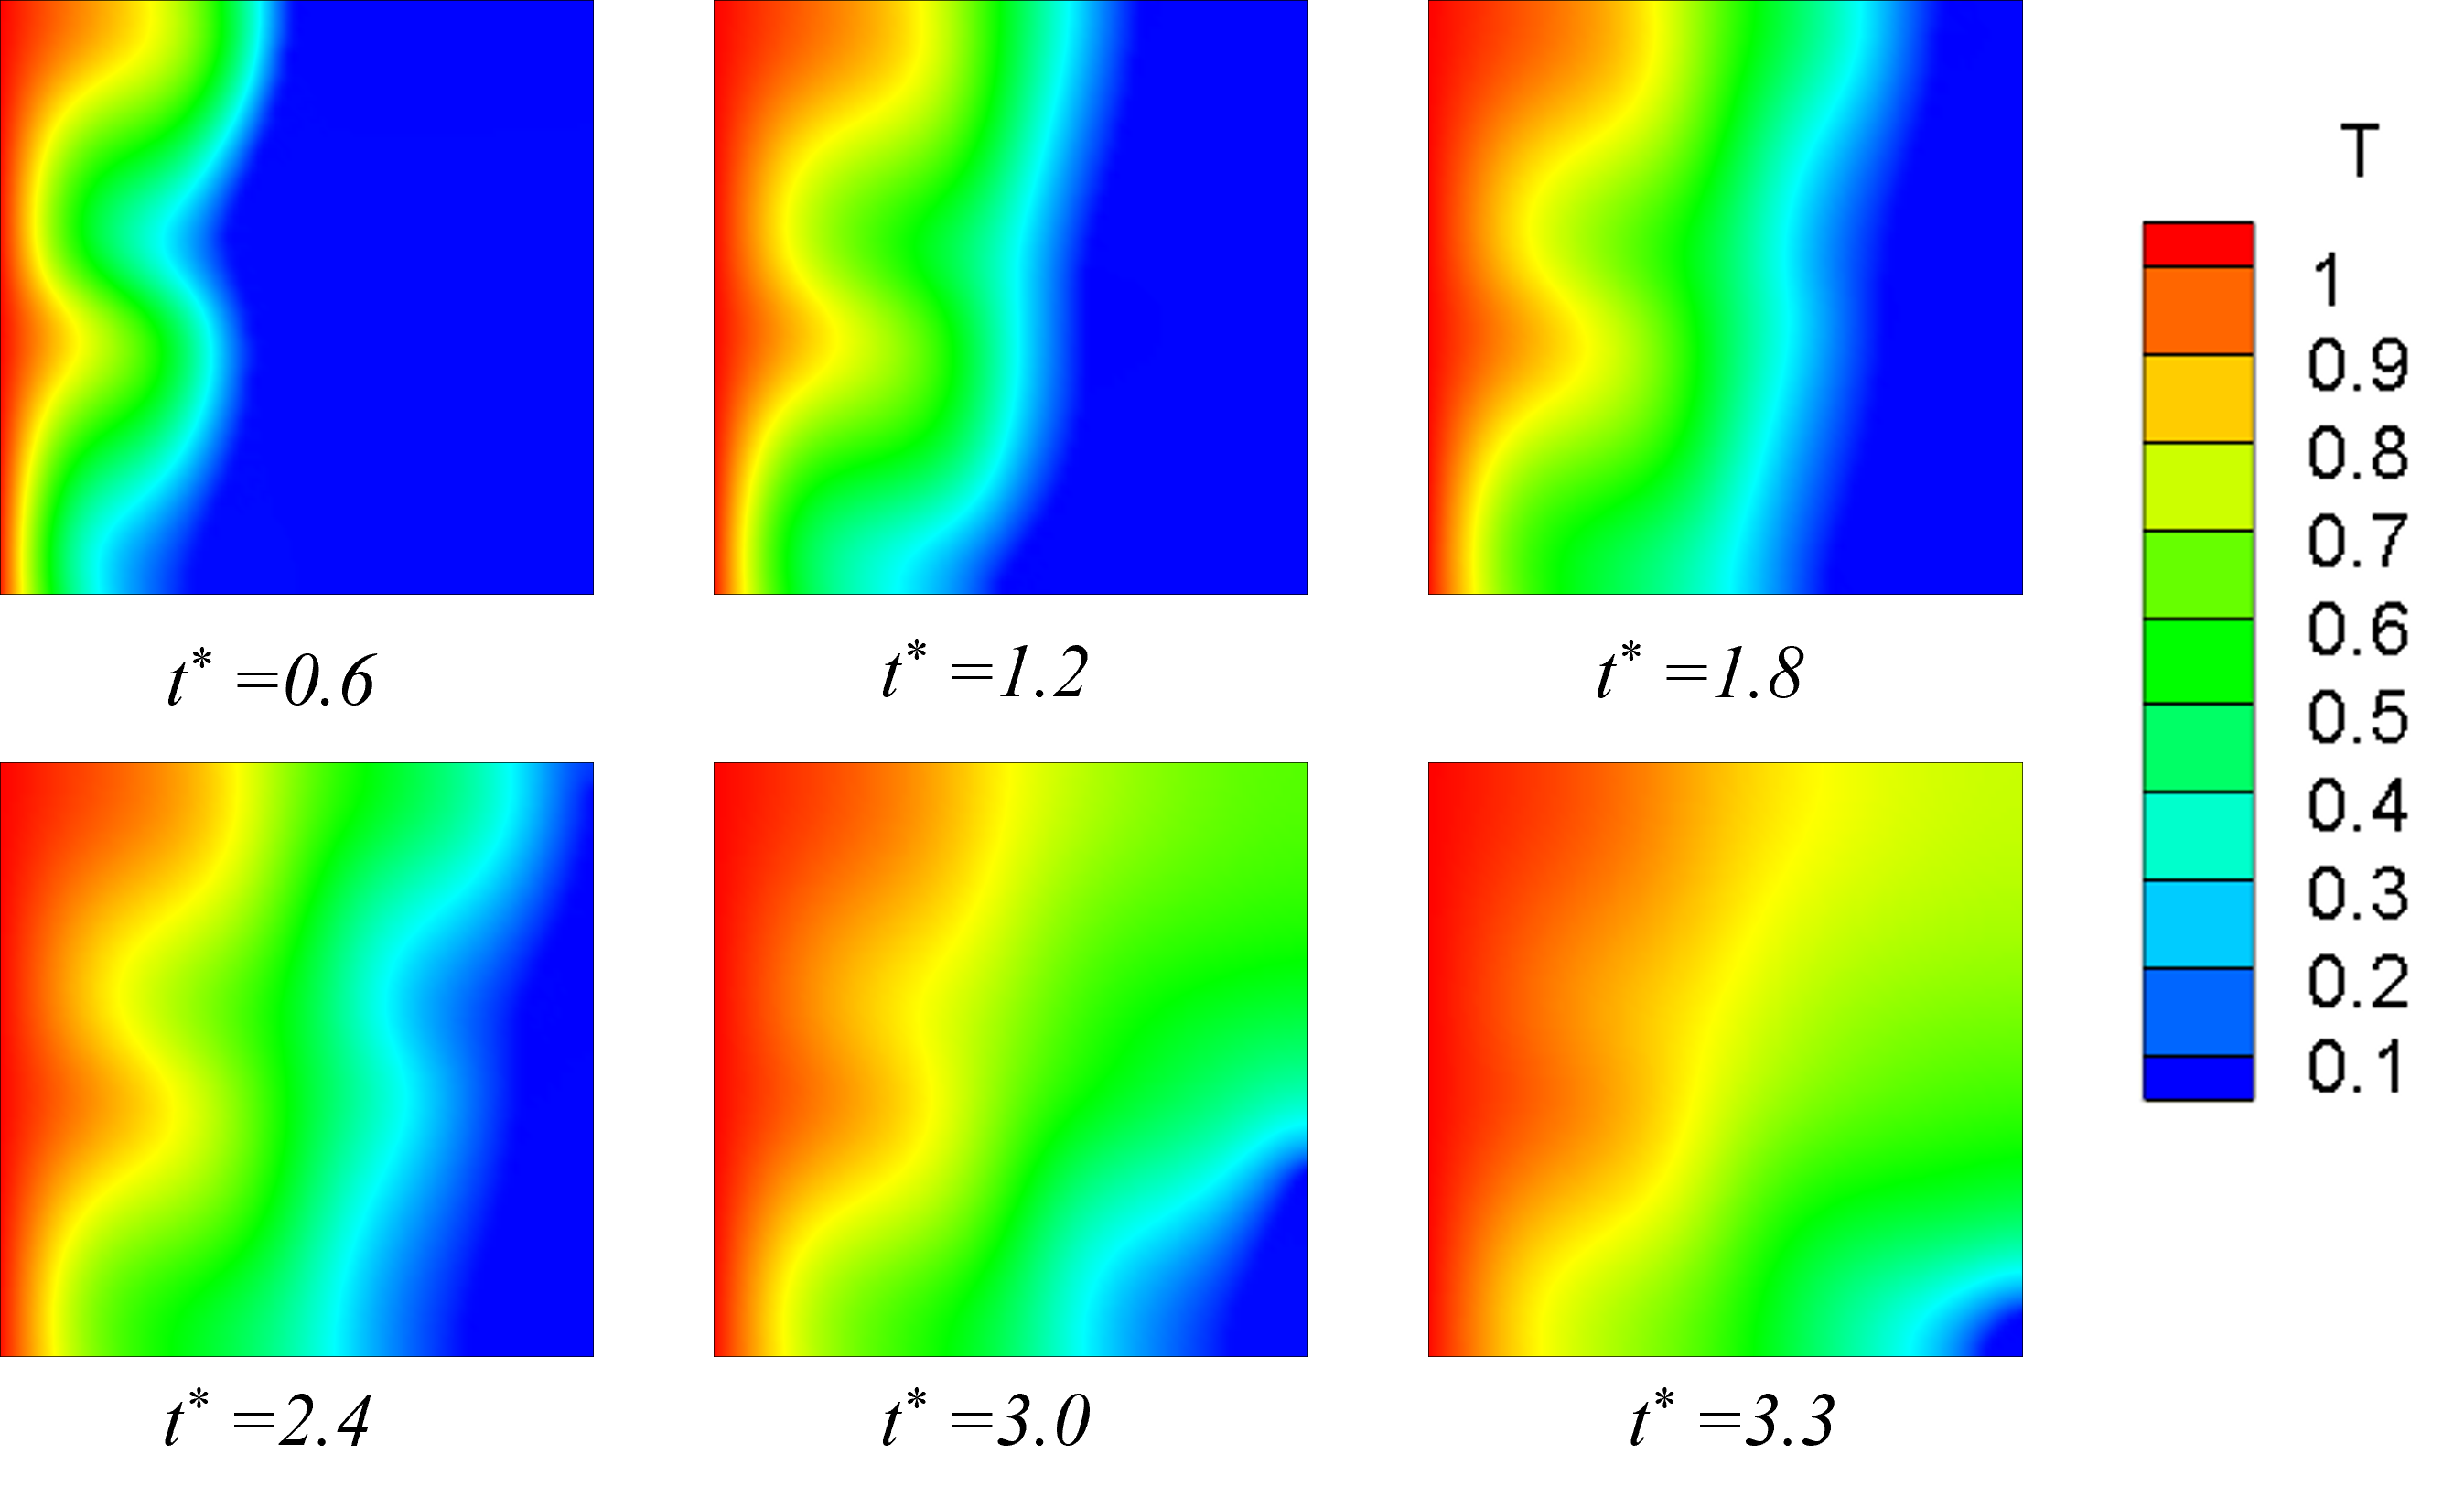
\includegraphics[scale=0.5]{Fig/yun1.png}
	\caption{The temperature distribution cloud of Type 1 at different $ t^* $} 
	\label{Fig_yun1} 
\end{figure}

Fig.\ref{Fig_sigma-T} graphically depicts the trend of the standard deviation of the temperature inside the model for the three distributions, and it is clear that there is an extremely large value. That is, the standard deviation of the temperature metropolis shows two phases: a sharp increase and a rapid decrease.In the process of heat transfer from the left wall to the interior, the internal PCM absorbs heat in the form of sensible heat, resulting in a local temperature rise. In the initial stage the temperature of the internal nanofluid is kept at $ T_0 $. When the internal temperature reaches the phase change temperature, the PCM inside the square cavity absorbs heat and transforms from the solid phase to the liquid phase. And the liquid fraction rises rapidly, and when the PCM close to the left wall partially melts, the remaining PCM mainly absorbs heat in the form of sensible heat, and the liquid fraction rises at a slower rate.
When the temperature of the part away from the left wall is still retained at the initial temperature, the standard deviation of the temperature rises sharply. When the internal PCM reaches the phase change temperature, the PCM begins to absorb a large amount of heat in the form of latent heat. Since the temperature of the phase change process remains near the phase change temperature, the standard deviation of the temperature starts to decrease.In the low Rayleigh number case, the main mode of heat transfer is thermal conductivity, while in the high Rayleigh number case, the main mode of heat transfer is heat convection, which results in a lower rate of increase of the average temperature in the low Rayleigh number compared to the high Rayleigh number, and the standard deviation of the temperature in the high Rayleigh number will rise in a shorter period of time, and the rate of decrease in the low Rayleigh number compared to the high Rayleigh number will be slower when reaching the phase change temperature.
	\begin{figure}[H]
	\centering
	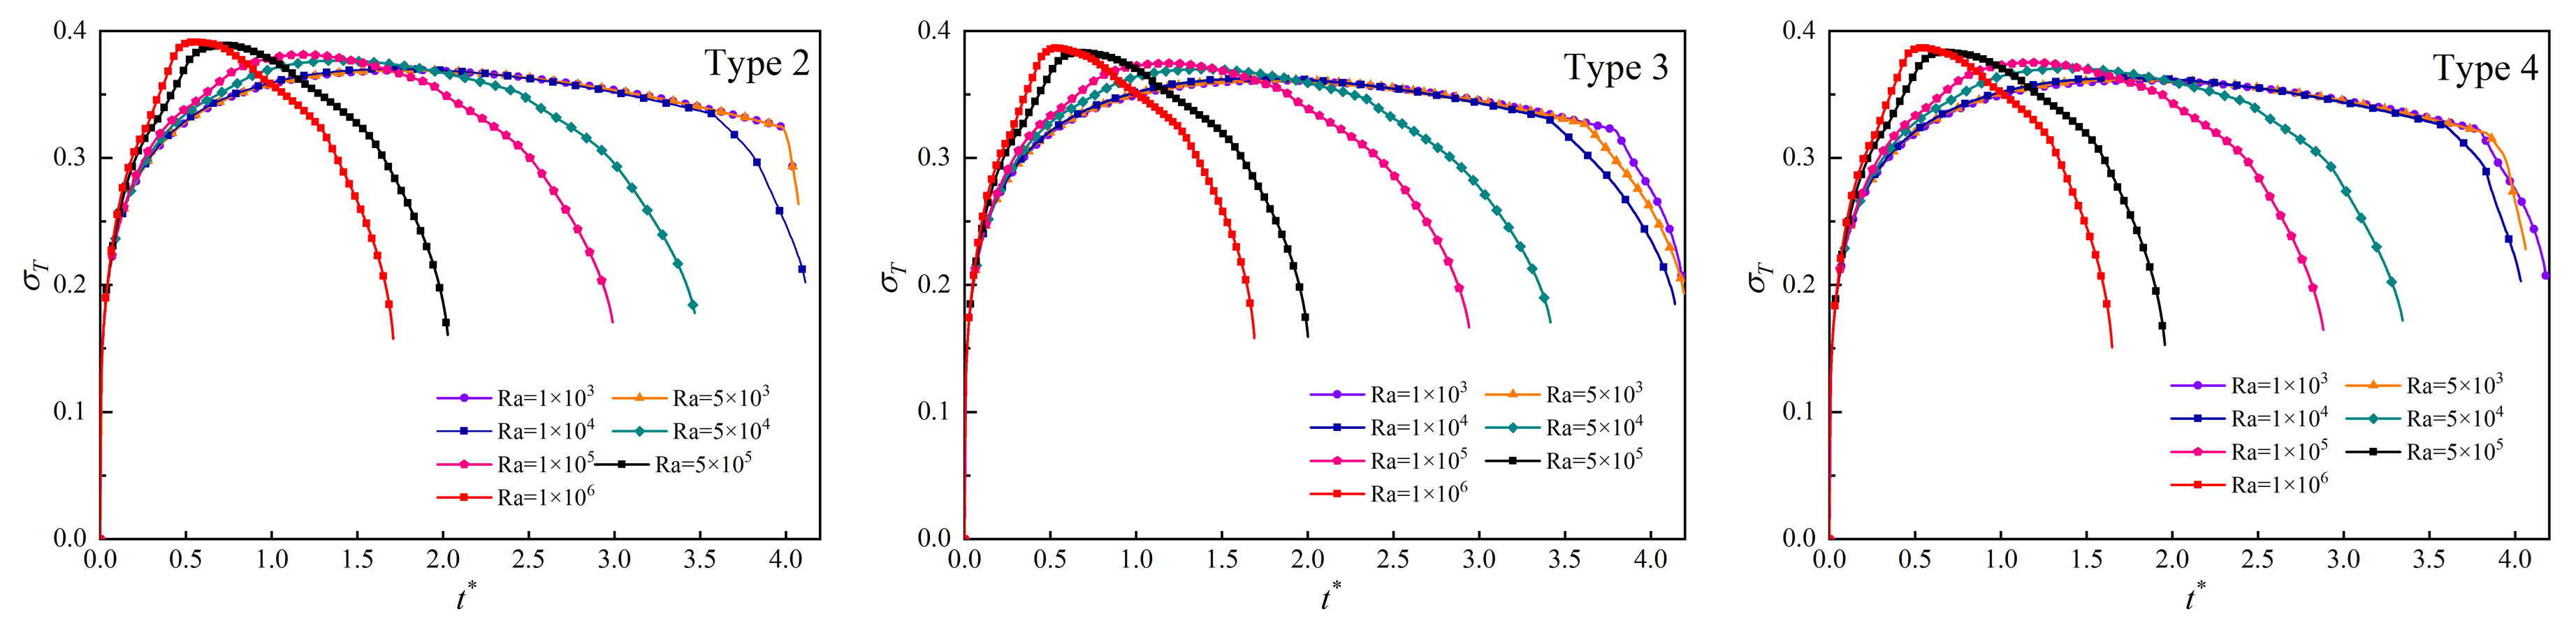
\includegraphics[scale=0.5]{Fig/sigma-T.png}
	\caption{Temperature standard deviation at $ t^* $ } 
	\label{Fig_sigma-T} 
\end{figure}

Average Nusselt number is calculated by:
\begin{equation}
	Nu_{ave}=-\int_0^1\left(\frac{\partial T^*}{\partial x^*}\right)_{x^*=0}dy^*
\end{equation}

The amount of the average Nusselt number reflects the strength of the fluid heat transfer. This is essential for understanding and optimising the heat transfer process. As an important index to evaluate the convection and thermal conductivity percentage of the system, it is crucial to analyse the average Nusselt number of the left wall surface with time for different Rayleigh numbers in this section. The Rayleigh number varies from $ 10^3 $ to $ 10^6 $. From the Fig.\ref{Fig_Nu}, it can be seen that in the case of small Rayleigh number, the proportion of thermal conductivity is relatively large, and the average Nusselt number does not rise very quickly. In the case of high Rayleigh number, convection is more important than heat conduction, so the average Nusselt number rises very quickly. The standard deviation of temperature decreases gradually as the melting proceeds and the convective heat transfer decreases gradually. The average Nusselt number decreases gradually, and the larger the Rayleigh number, the faster it decreases. 
\begin{figure}[H]
		\centering 
		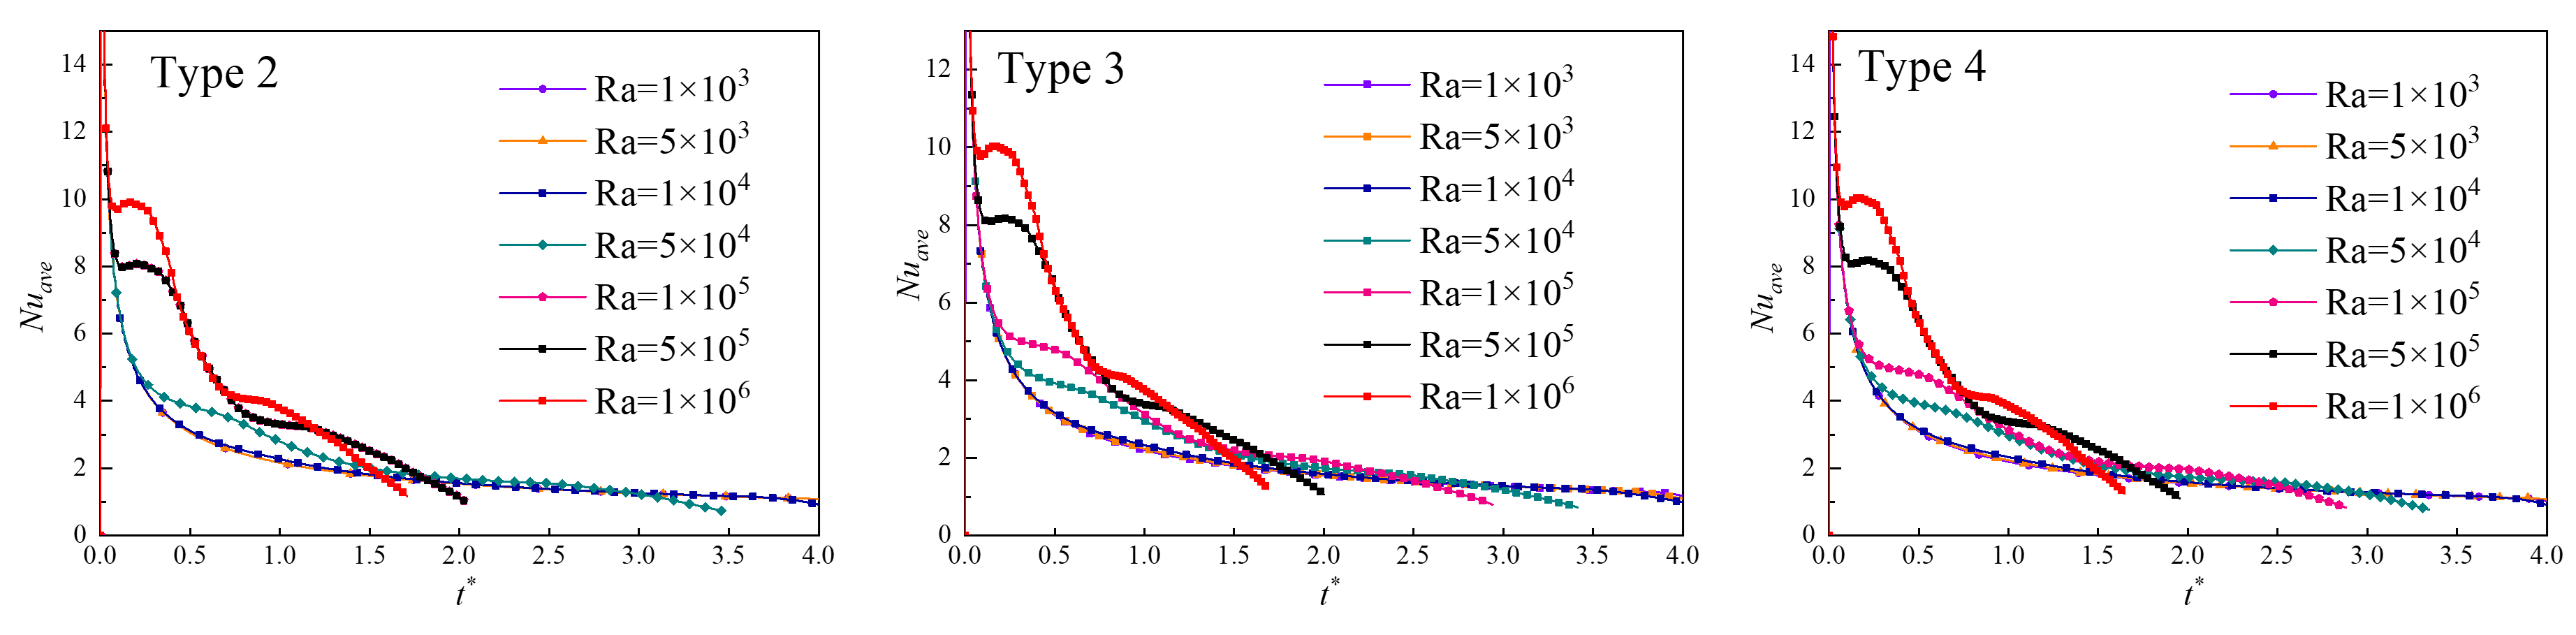
\includegraphics[scale=0.5]{Fig/Nu-t.png}
		\caption{Average Nusselt number at $ t^* $  } 
		\label{Fig_Nu} 
	\end{figure}

	\subsection{Effects of arrangement}

In this sub-section, the Al$_2$O$_3$ nanoparticle melting between various arrangement scenarios, the Al$_2$O$_3$ nanoparticle melting in each region in each arrangement scenario is investigated separately by monitoring the \textit{fl} parameter in each region. 
The Rayleigh number are set as $ 10^4 $. 
Other settings of the parameters and how the regions are divided and named are the same as in 3.1.
The regional concentrations of each type used in this section are shown in Table \ref{typee}.

\begin{table}[H]
	\centering
	\footnotesize
	\caption{Concentrations added by type and region}
	\begin{tabular}{cccccc}
		\toprule
		& Upper left  & Upper right  & Bottom left  & Bottom right  \\
		& concentration  & concentration  & concentration  & concentration  \\
		\midrule
		Type5 & 0.05 & 0.03  & 0.03   & 0.05   \\
		Type6 & 0.05 & 0.03  & 0.05   & 0.03   \\
		Type7 & 0.05 & 0.05  & 0.03   & 0.03   \\
		\bottomrule
	\end{tabular}
	\label{typee}		
\end{table}

\subsubsection{Effects of arrangements between layouts}
This subsection focuses on Types 1-4. Fig.\ref{Fig_fl} shows the variation of liquid fraction with dimensionless time for each part when Rayleigh number equals to $ 10^4 $. Fig.\ref{Fig_yun2}  illustrates the temperature counters for type 2-4 at \textit{$ t^* $} = 1.0, 2.0, 3.0, and 4.0.

Combined with the counters it can be analyzed that the upper left region under the three distributions melts the fastest and reaches the \textit{fl} = $ 1 $ at \textit{$ t^* $} = $ 0.9714 $, $ 0.9714 $ and $ 0.93616 $ respectively, followed by the lower left part of the region, which reaches the liquid fraction = 1 at \textit{$ t^* $} = $ 1.21317 $, $ 1.09475 $ and $ 1.27317 $. In the process of melting of the two left regions the nanoparticles in the two right regions hardly melted. The melting tendency of the right two regions occurs only when the left region is nearly completely melted. The upper right region reaches the liquid fraction = $ 1 $ at the dimensionless time, and the lower right region reaches the liquid fraction = $  1 $ at the dimensionless time, respectively. Under the effect of thermal expansion of the liquid, the heated fluid will be subject to buoyancy and flow upwards, forming a natural convection in a clockwise direction, with the phenomenon of fast melting in the upper part and slow melting in the lower part. The yellow curve in the figure represents the change of the average liquid fraction in the four regions, and it is obvious to see that the two regions on the right are the main factors affecting the melting rate.

\begin{figure}[H] 
	\centering
	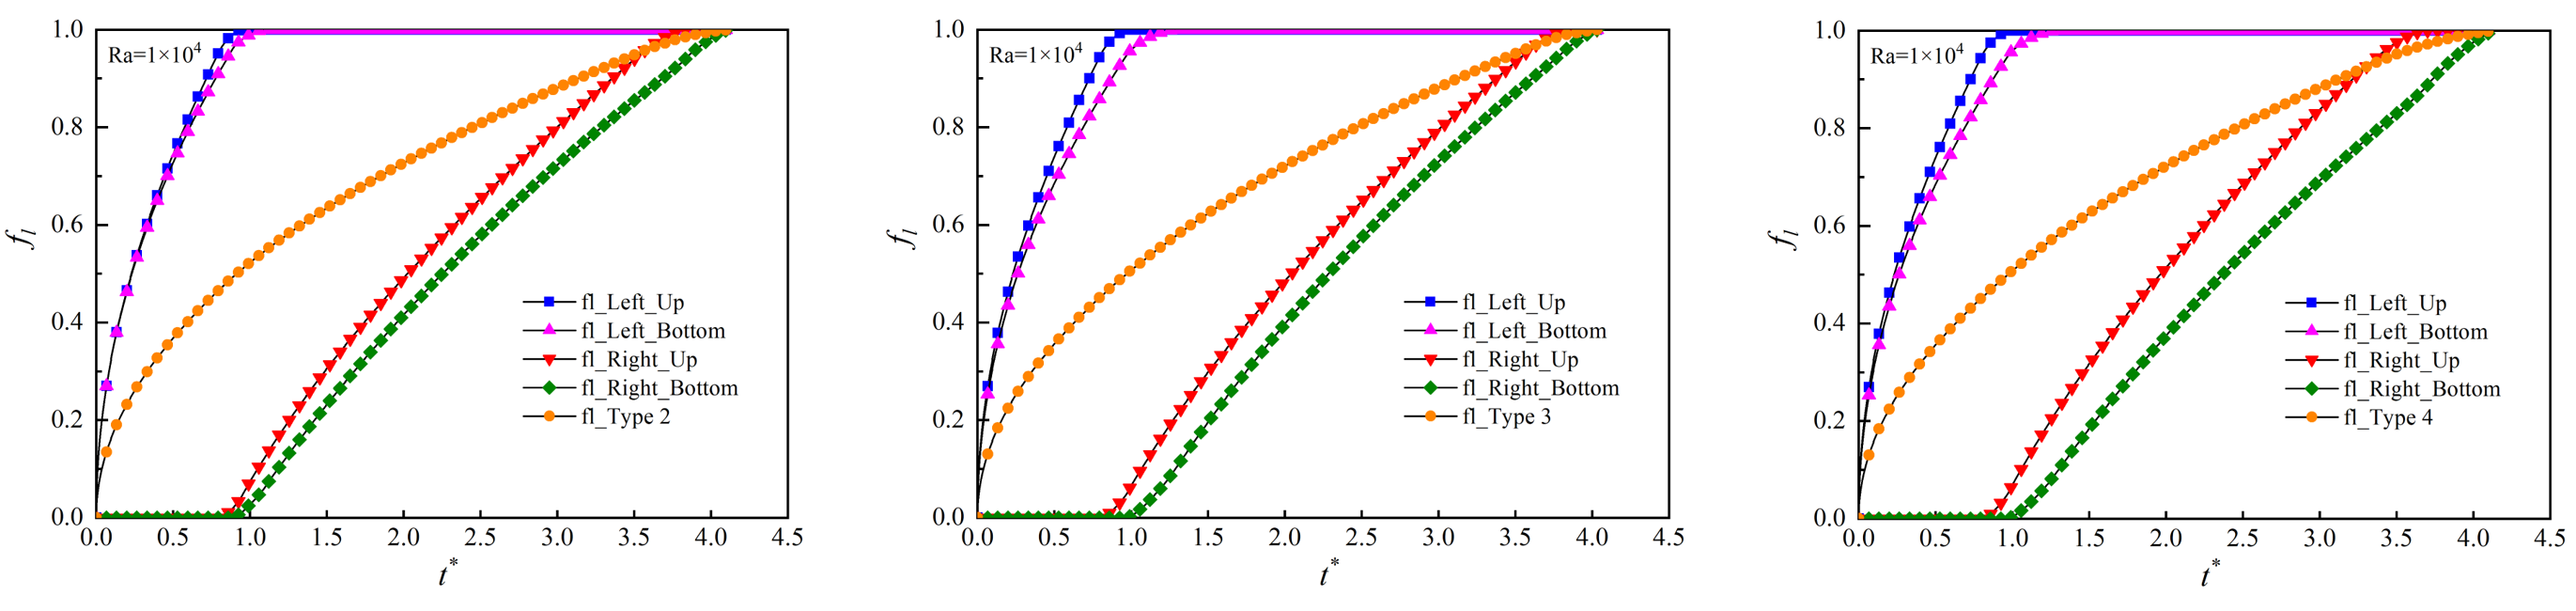
\includegraphics[scale=0.65]{Fig/fl2.png}
	\caption{Variation of \textit{fl} at $ t^* $ between layouts } 
	\label{Fig_fl} 
\end{figure}
The variation rule of Al$_2$O$_3$ nanoparticle melting with dimensionless time in each region under various arrangements is the focus of the investigation. 
\begin{figure}[H]
	%\noindent
	\centering 
	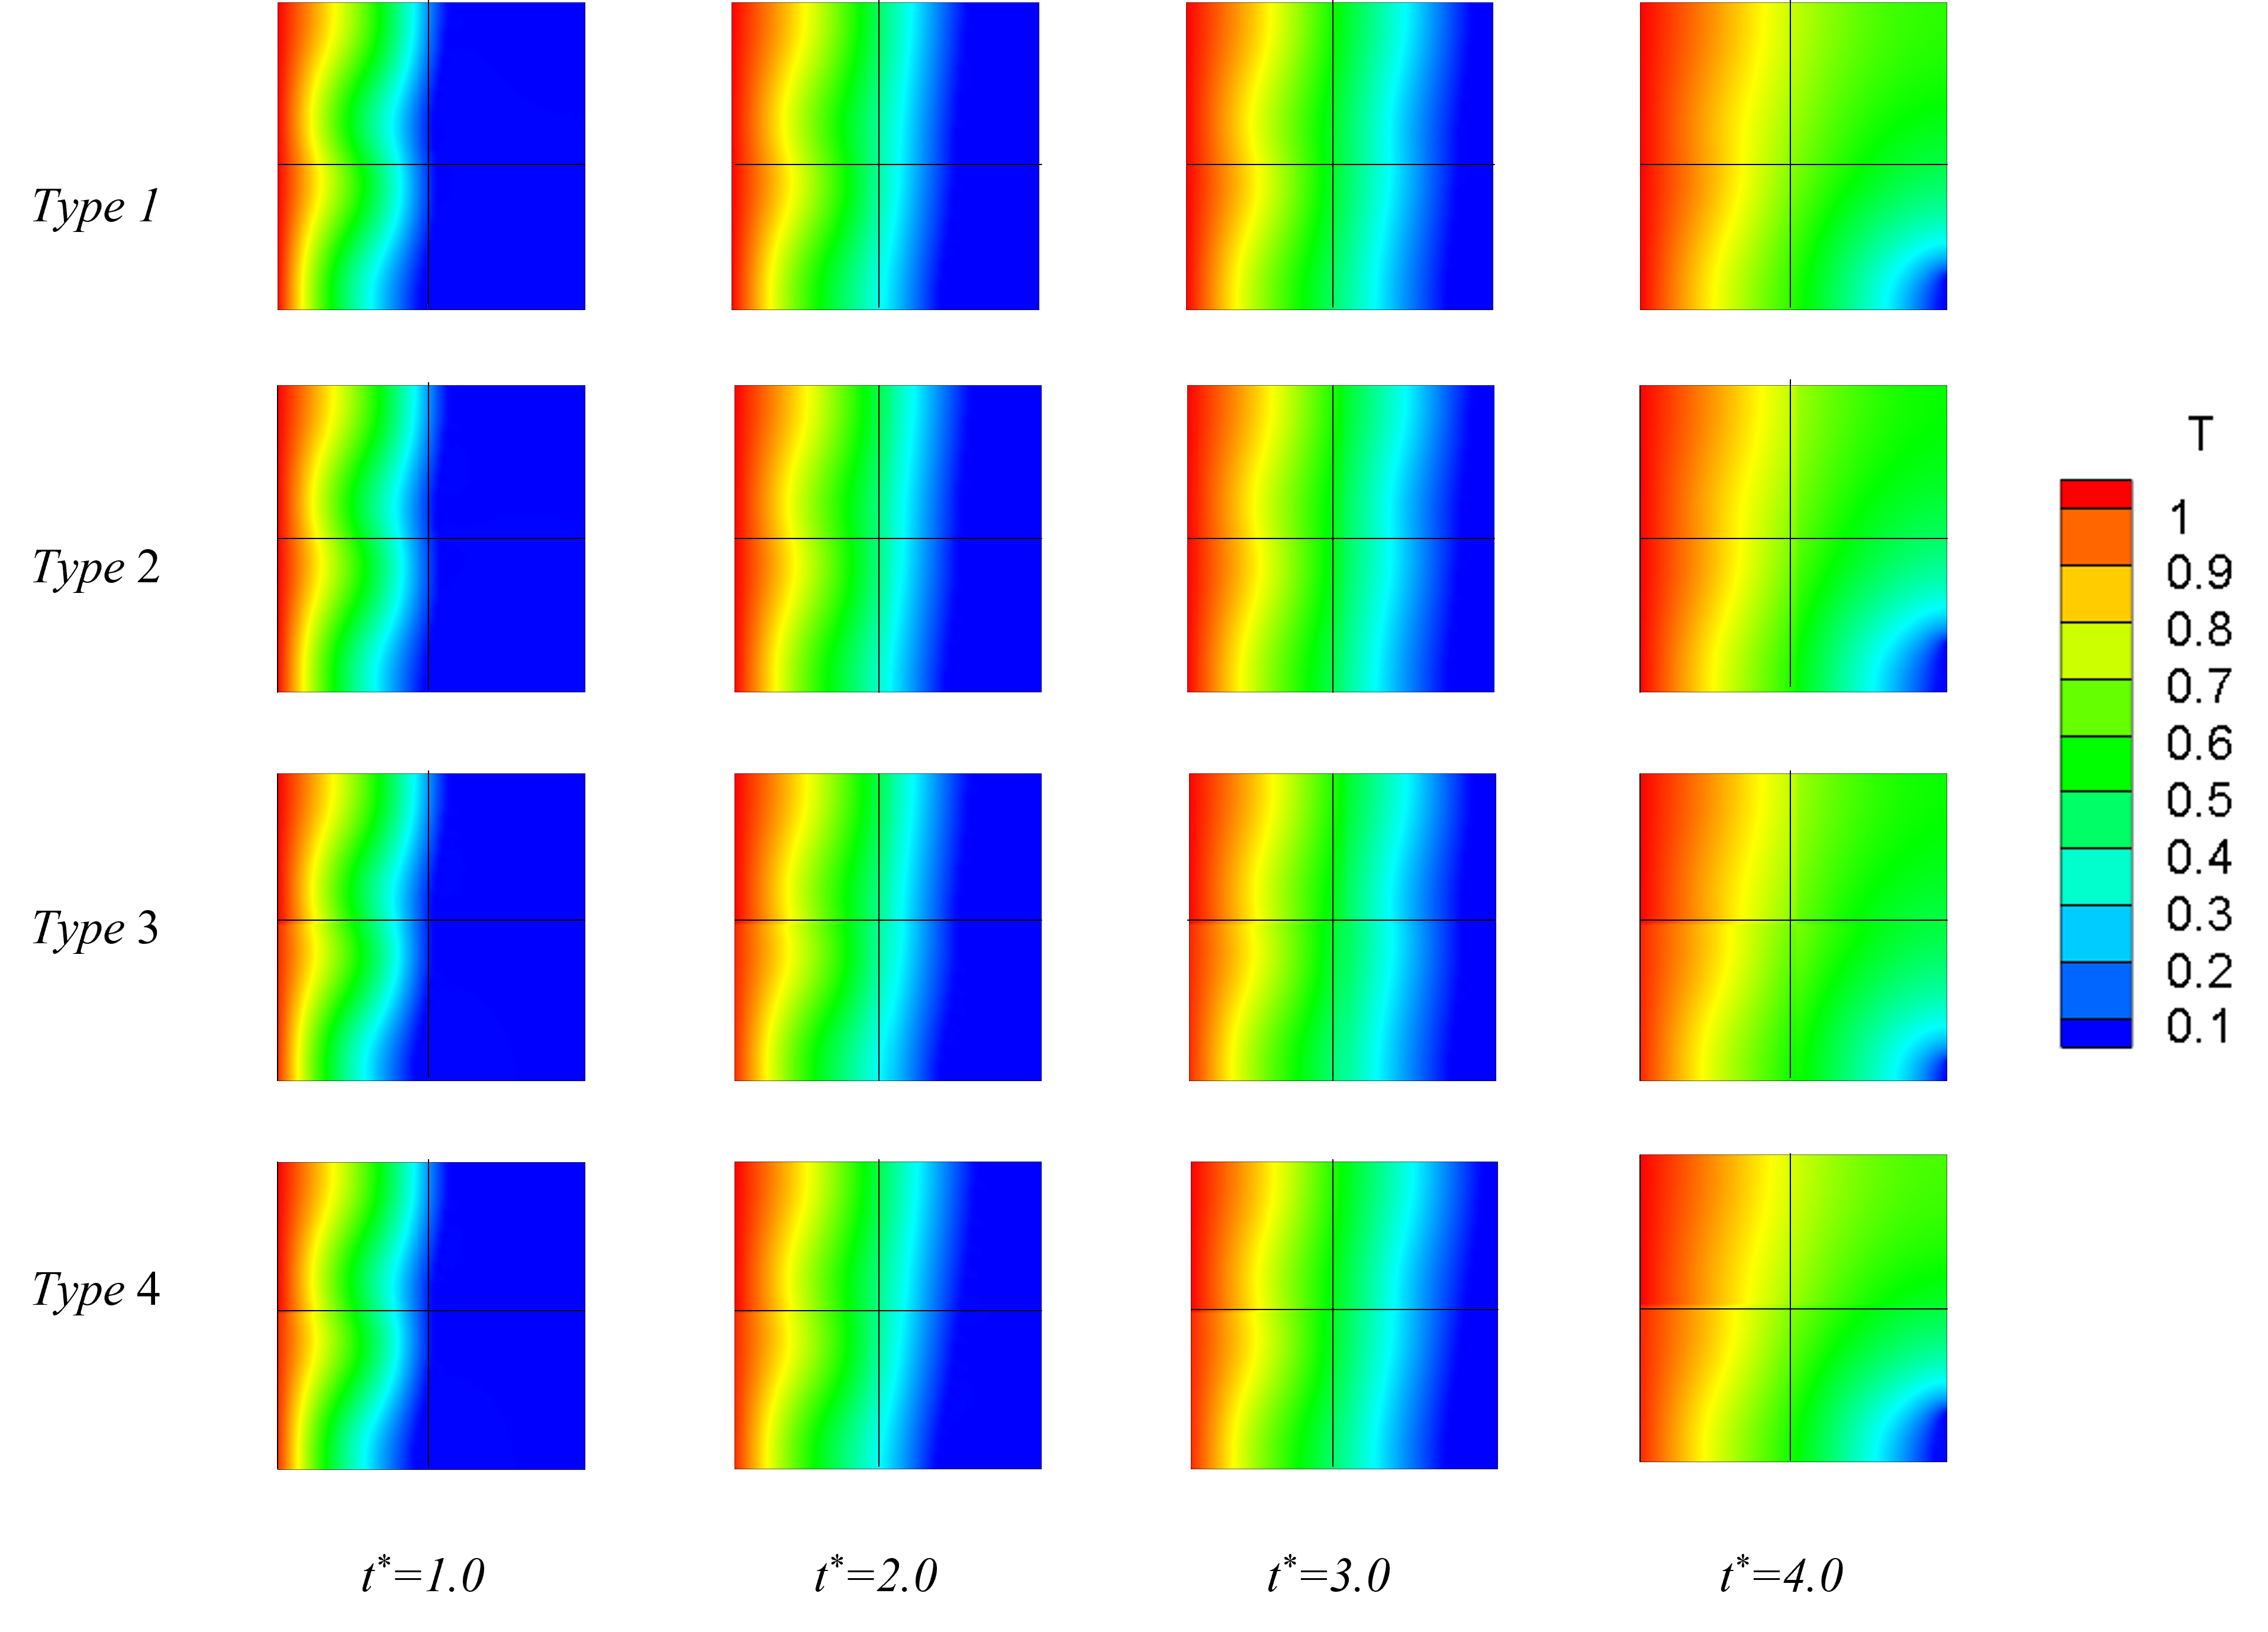
\includegraphics[scale=0.4]{Fig/yun2.png}
	\caption{Distribution of cloud maps of types 2-4 at $ t^* $} 
	\label{Fig_yun2} 
\end{figure}

\subsubsection{Effects of arrangements within layouts}
This subsection focuses on Types 1-7. Fig.\ref{Fig_fl2} illustrates the variation of the \textit{fl} with dimensionless time for various cases with Rayleigh number equals to $ 10^4 $. Fig.\ref{Fig_yun3}  illustrates the temperature cloud for type 5-7 at \textit{$ t^* $} = 1.0, 2.0, 3.0, and 4.0. 

Combined with the cloud counters it can be analyzed that the rate of increase of the liquid fraction for type 2-4 are greater than those of the control group in the upper left corner region. Because convective heat transfer is more pronounced in the upper left region, its melting is faster. 
Type 5-7 all have a lower rate of increase in the liquid fraction than the control because their nanoparticle volume fractions are larger so their melting is slower.
In the lower left region, the rate of increase of the liquid fraction of type 2,6 and 7 are greater than that of the control group. Because of its more pronounced ability to conduct heat and transfer heat, it melts faster.
In the upper right region, the liquid fraction increase rates of Type 4,5 and 6 are greater than those of the control group. Due to their smaller nanoparticle volume fraction, they melt faster.
In the lower right region, the rate of increase of liquid fraction for types 2,3 and type 7 are greater than that of the control group. It melts faster because it is subjected to stronger upper convection and left conductive heat transfer.
\begin{figure}[H]
	\centering
	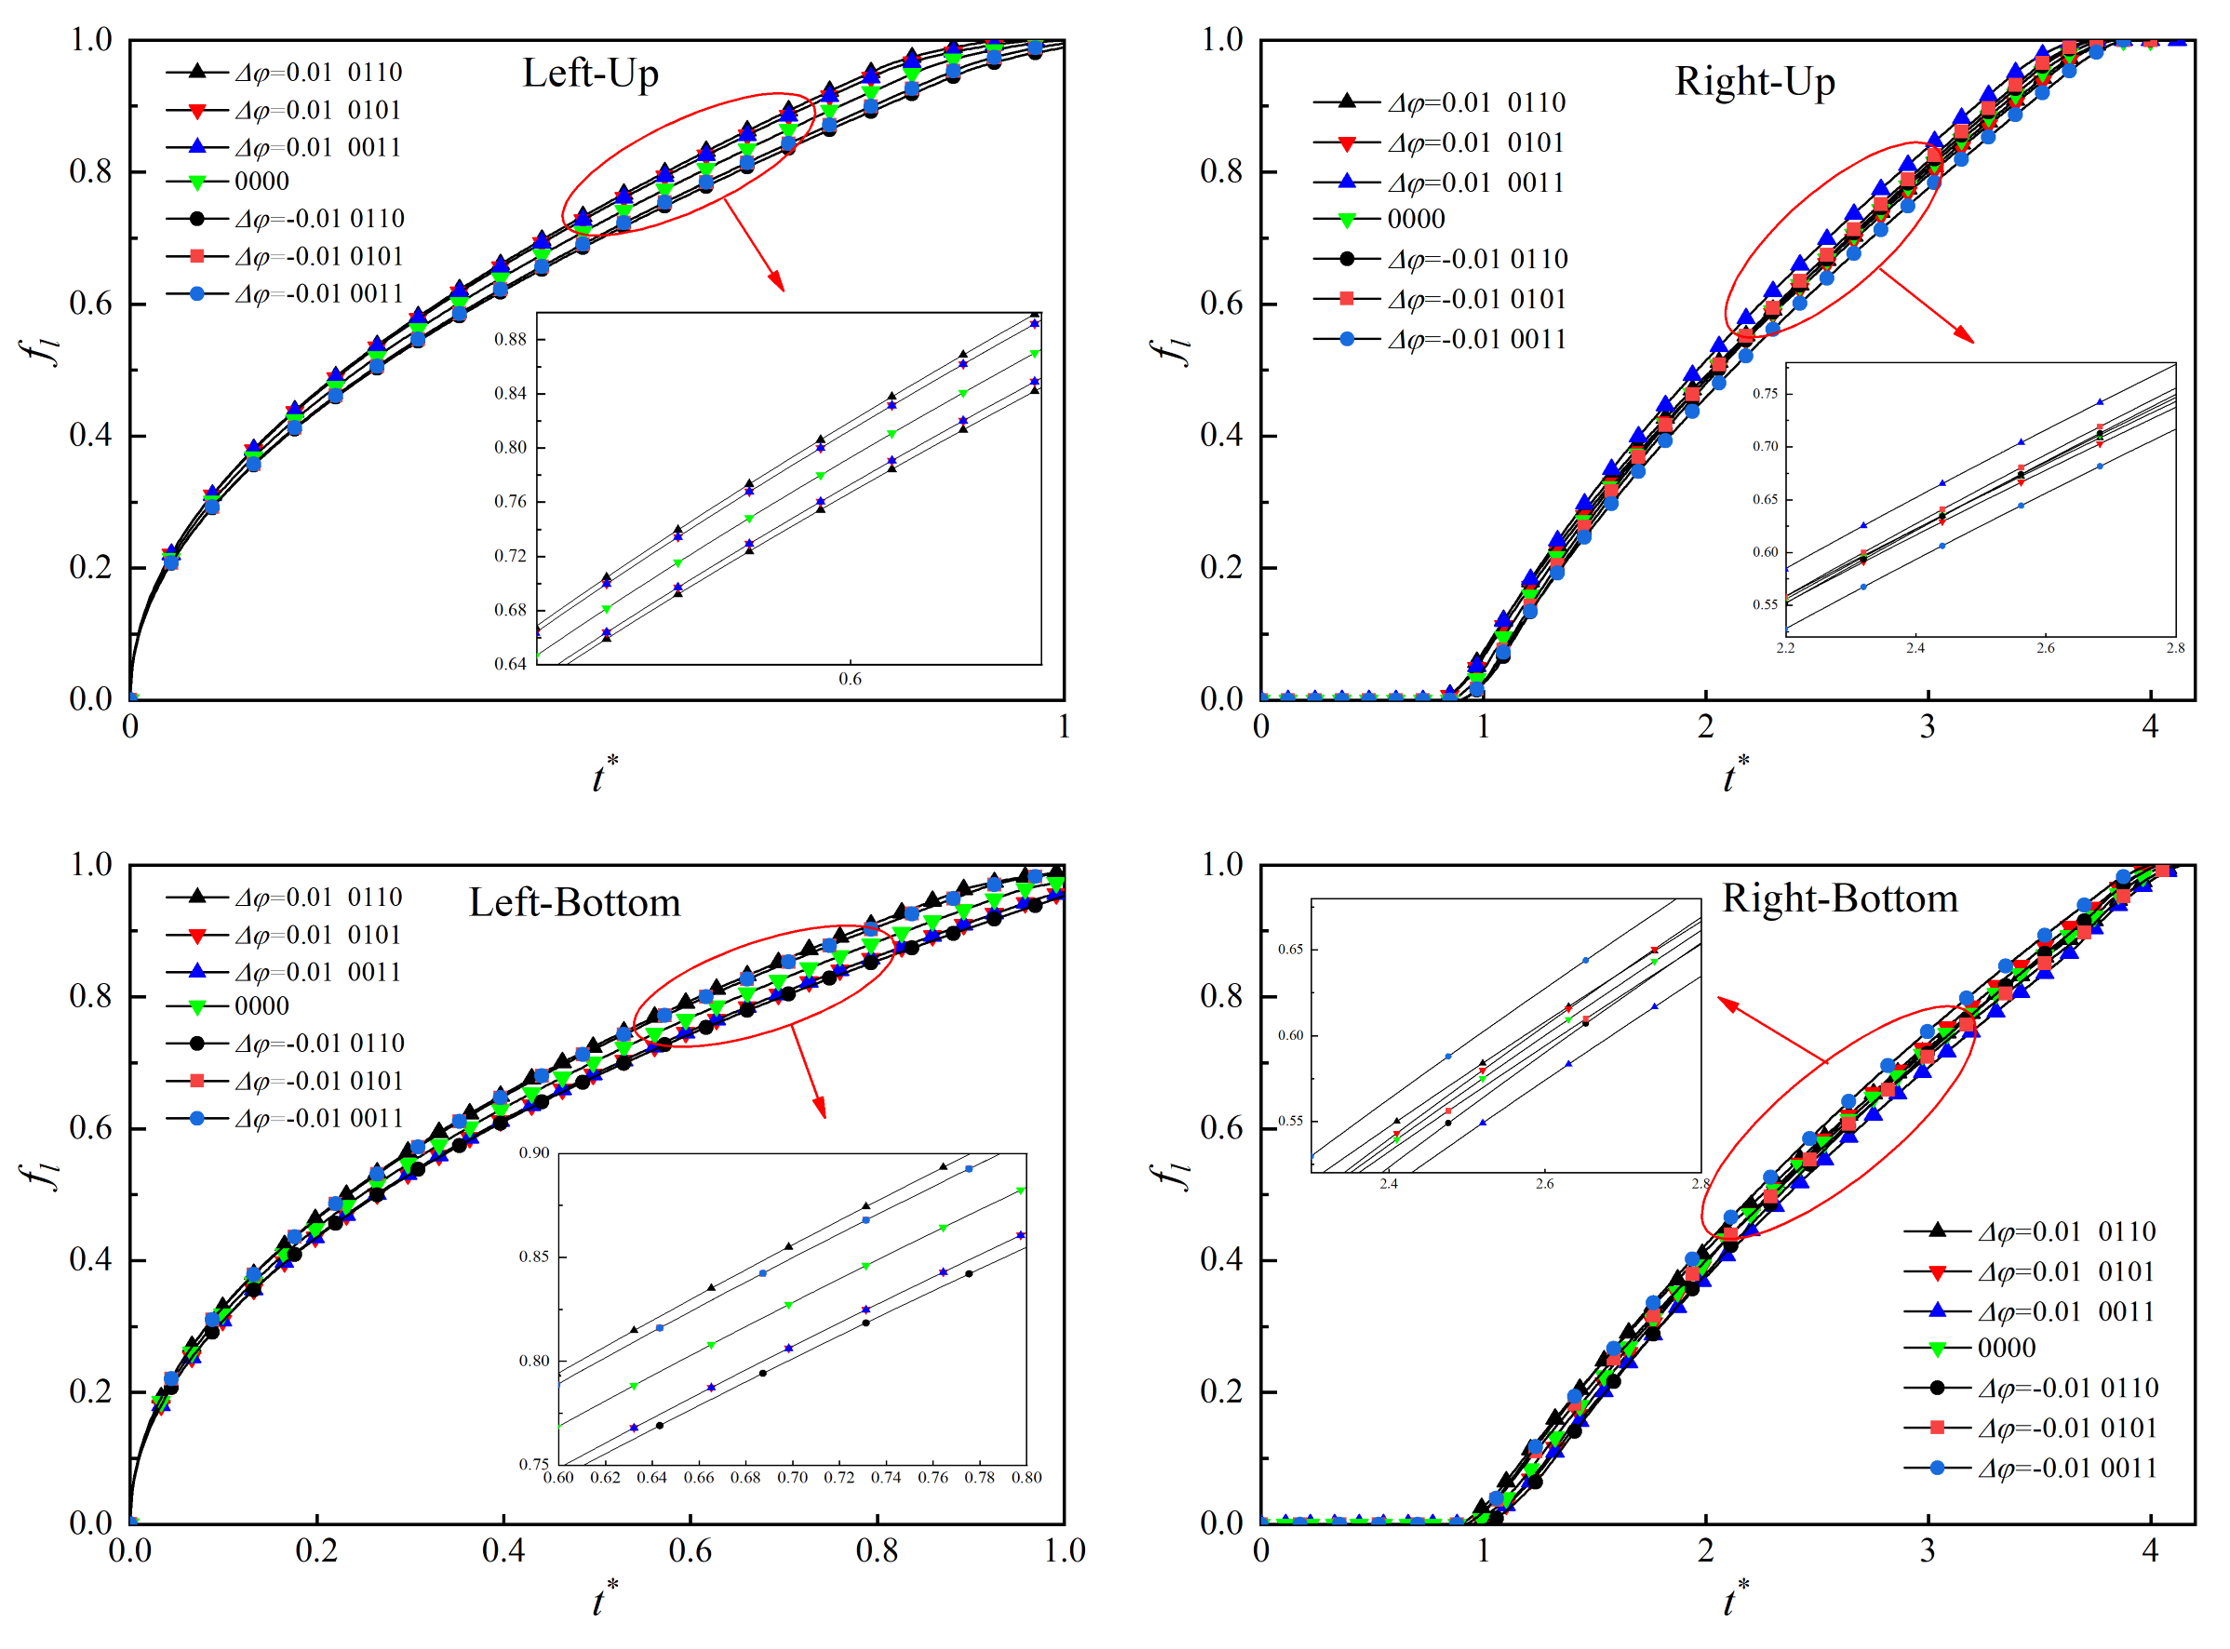
\includegraphics[scale=0.6]{Fig/fl.png}
	\caption{Variation of \textit{fl} at $ t^* $ within layouts}
	\label{Fig_fl2} 
\end{figure}

\begin{figure}[H]
	\centering
	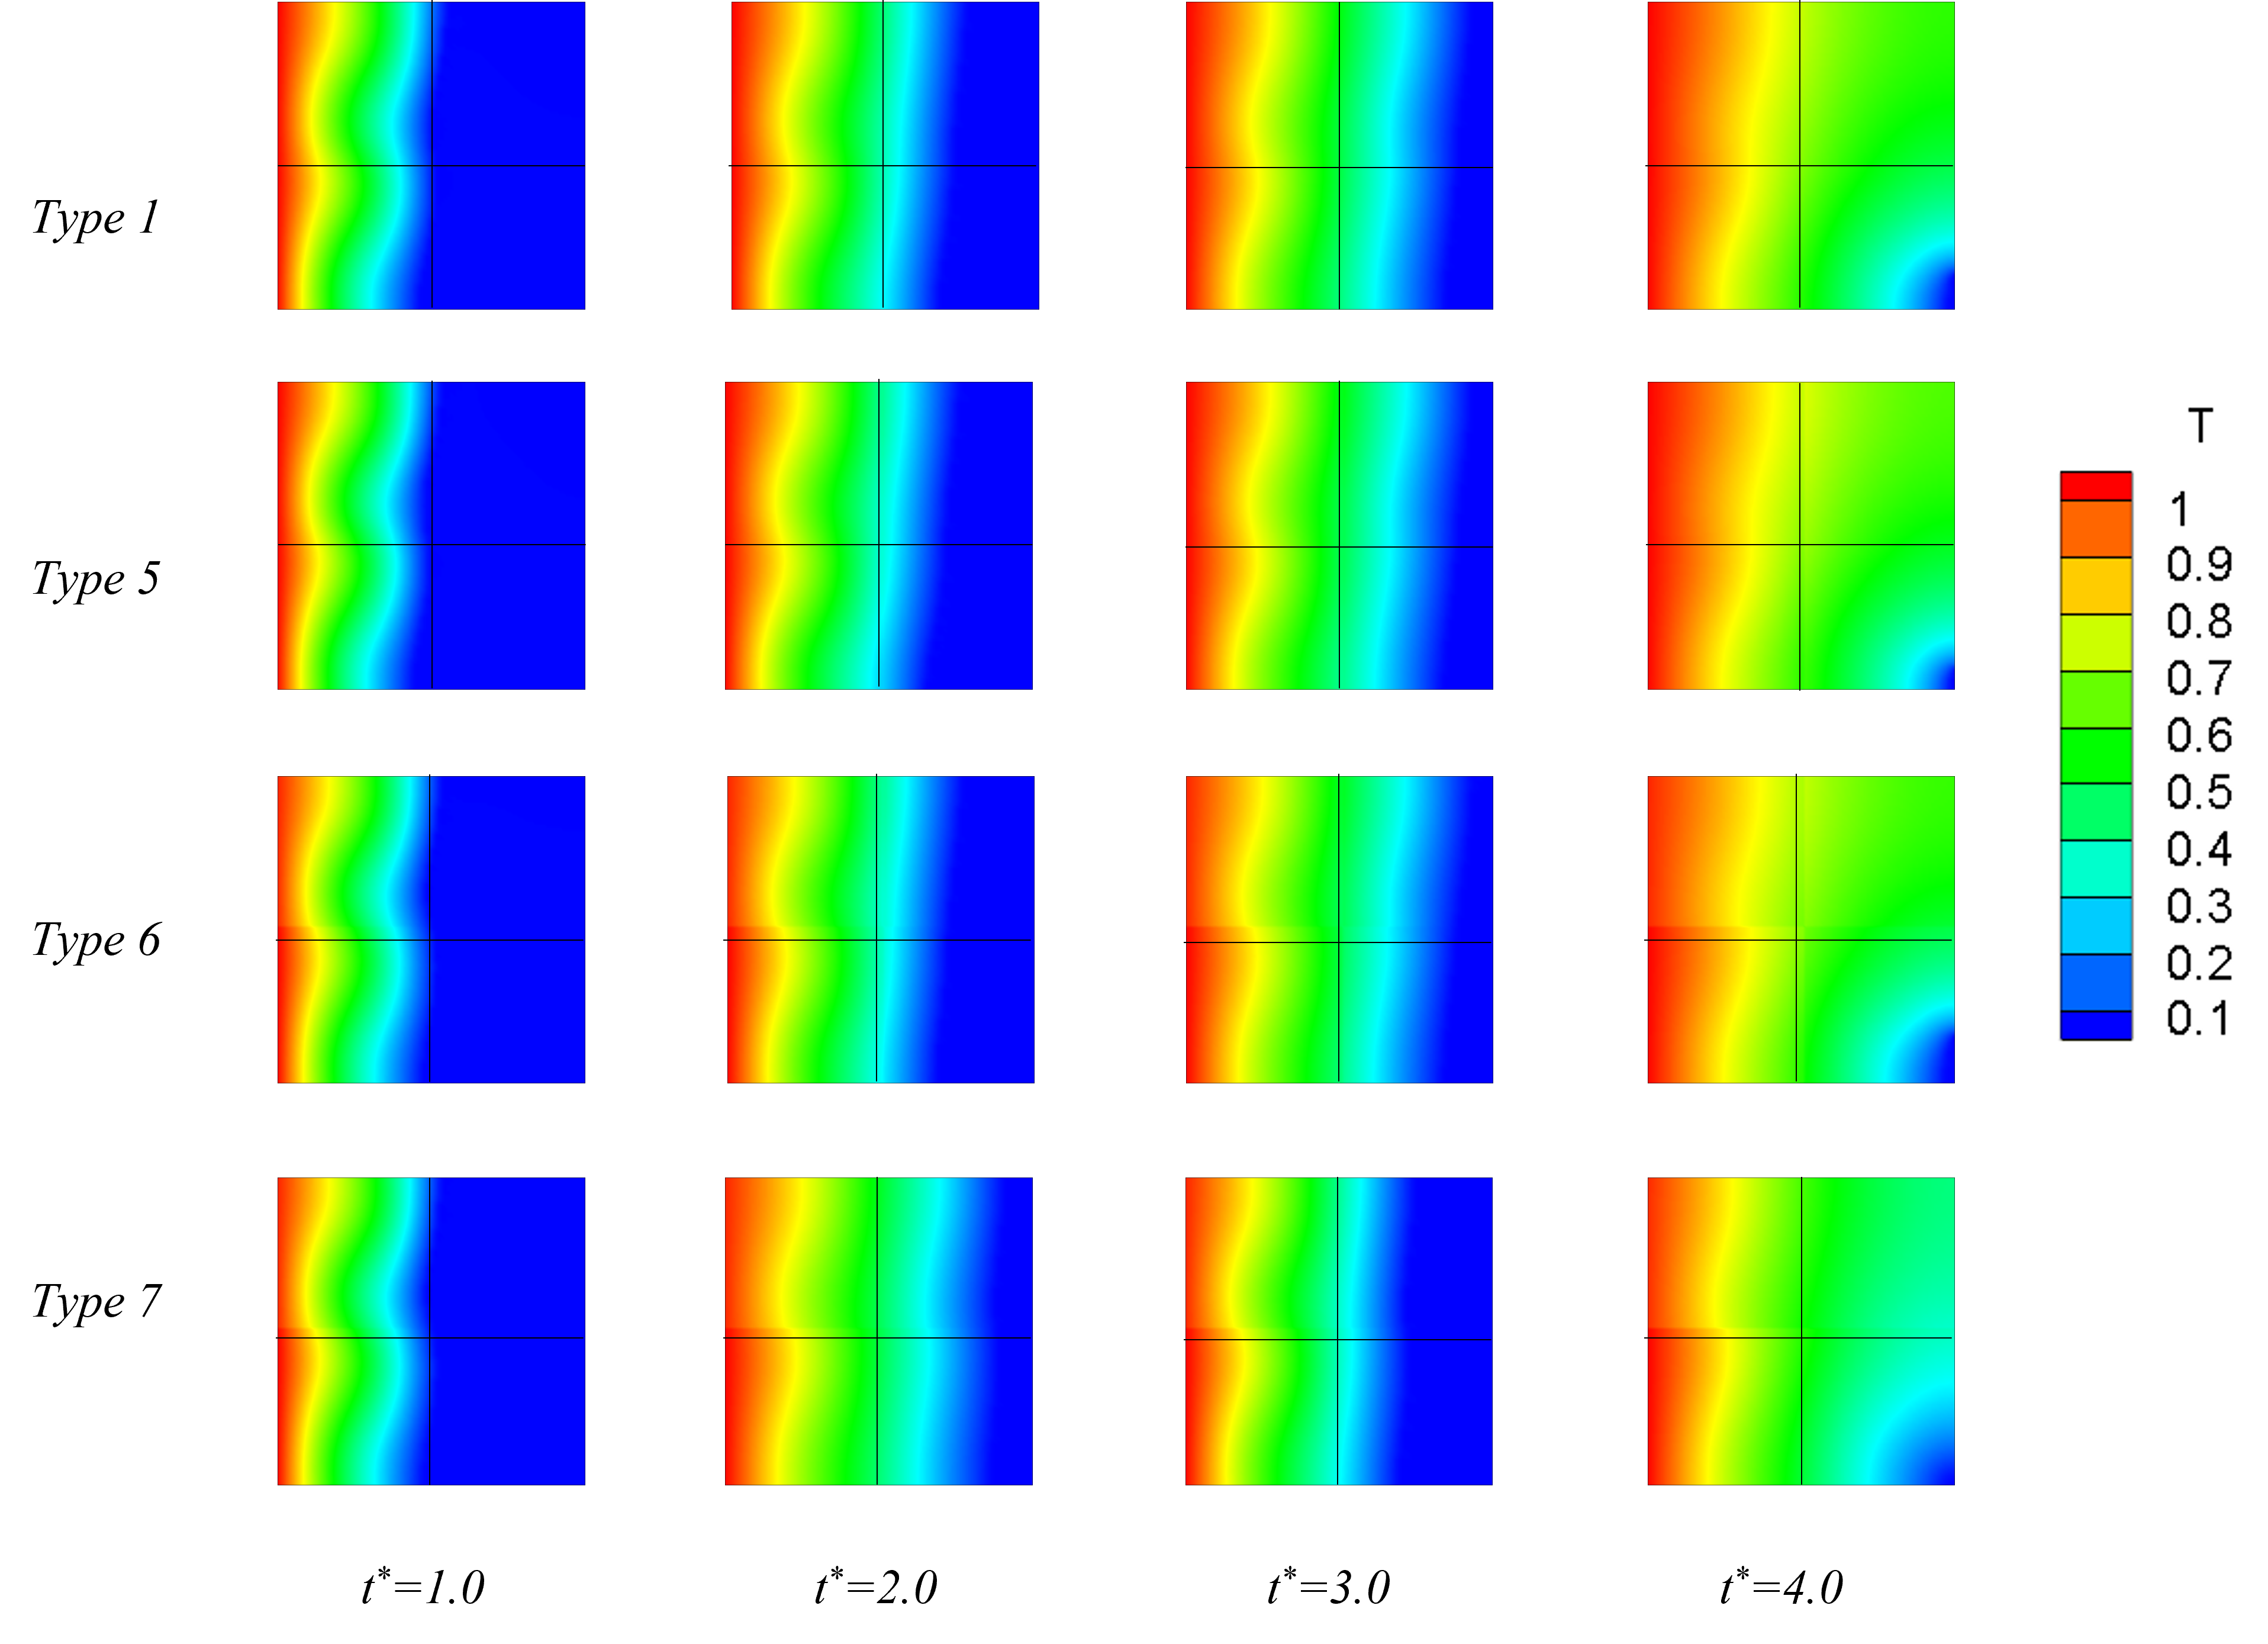
\includegraphics[scale=0.4]{Fig/yun3.png}
	\caption{Variation of \textit{fl} at $ t^* $ within layouts}
	\label{Fig_yun3} 
\end{figure}
For the research to determine the melting of the upper and lower, left and right parts of the square cavity region.
The liquid fractions of  the left, right, top and bottom parts were analysed.

The ratio of the left and right parts is calculated by:
\begin{equation}
	K_1=\dfrac{fl_{Right-Up}+fl_{Right-	Bottom}}{fl_{Left-Up}+fl_{Left-Bottom}}
\end{equation}

The ratio of the up and bottom parts is calculated by:
\begin{equation}
	K_2=\dfrac{fl_{Right-	Bottom}+fl_{Left-Bottom}}{fl_{Right-Up}+fl_{Left-Up}}
\end{equation}

As can be seen from Fig.\ref{ratio}, $ K_1 $ shows an increasing trend while $ K_2 $ shows a decreasing and then increasing trend, $ K_1 $ shows an increasing trend because the heating of the left wall makes the melting rate of the left PCM relatively fast; with the convective convection, the PCM of the right part melts slowly to all melting, and$  K_1 $ reaches 1. $ K_2 $ shows a decreasing and then increasing trend is because at the beginning of the two parts of the right side of the liquid fraction are 0, the liquid fraction of the two regions on the left side of the influence of thermal conductivity to maintain almost the same rate of melting; as convective heat transfer to carry out the arrival of the heat gathered in the upper part of the left upper part of the heat than the sitting down part of the accumulation of heat faster, so that the rate of melting to speed up the $ K_2 $ shows a decline; the types in the t * = 0.80399 , 0.8084, 0.8084, 0.84805, 0.89431, 0.8899, and 0.8899 onwards, the tendency for the upper right corner to melt first than the lower right corner and for the \textit{fl} to be larger resulting in a decrease in $ K_2 $ decreases, and with the continuation of melting at t*=0.8062, 0.9692, 1.23352, 1.38551, 1.36349, 3.4803, 1.26877 began to rise slowly until it reached 1. $\Delta\varphi$ = $ -0.01 $ Under types 3 and 4 at the beginning $ K_2  $ is greater than 1 because the lower part of the seat is more thermally conductive than the upper left part.
\begin{figure}[H]
	\centering
	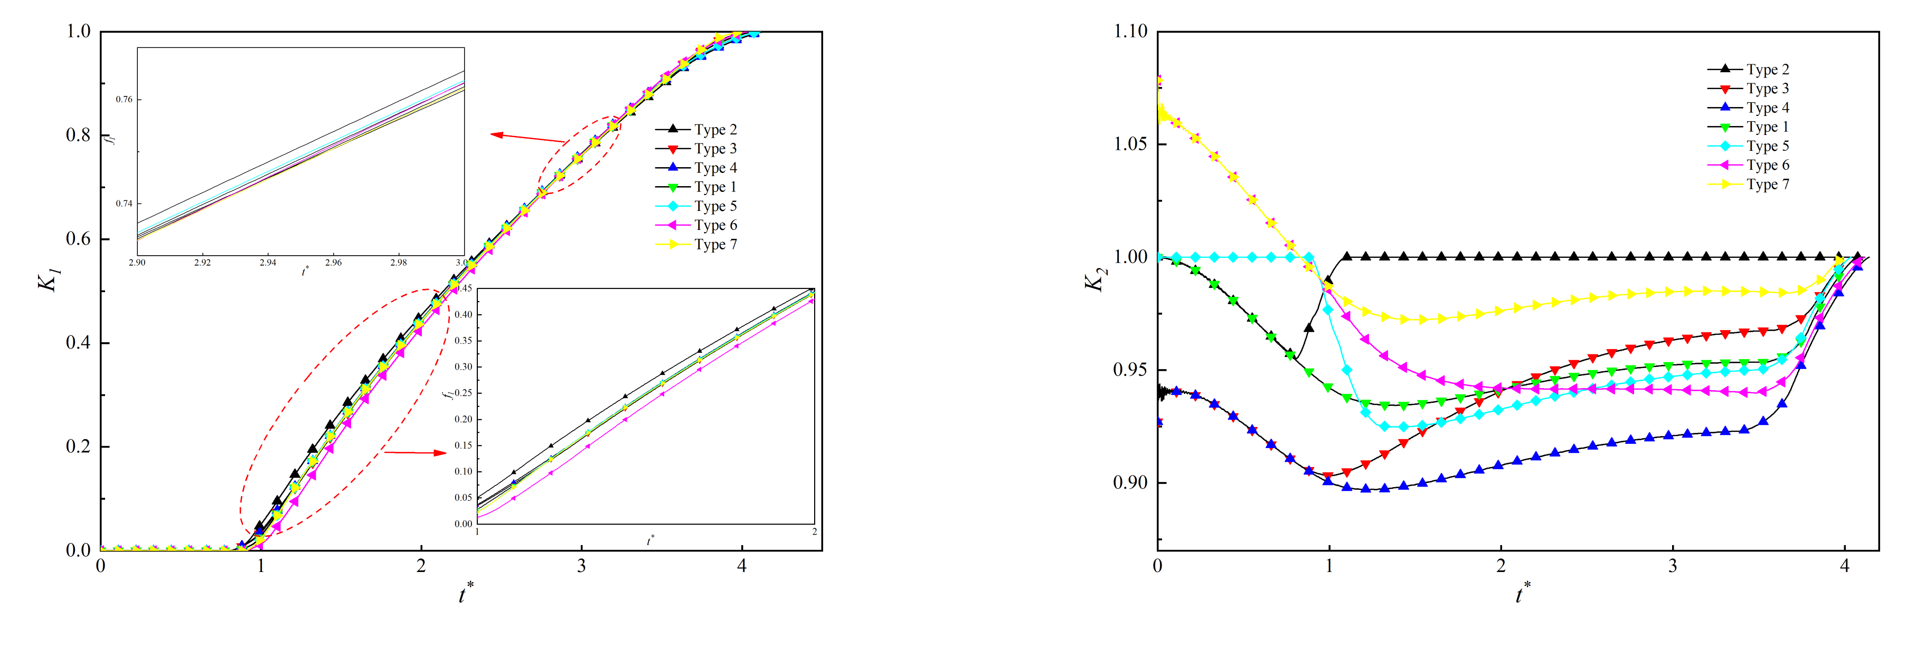
\includegraphics[scale=0.9]{Fig/ratio.png}
	\caption{Ratio of left-to-right and top-to-bottom \textit{fl}s at $ t^* $}
	\label{ratio} 
\end{figure}


	\subsection{Effects of volume fraction}

In this section, the melting characteristics of nanoparticles with the same volume fraction but different volume fractions of each part of the structure are investigated using the model shown in Figure \ref{Fig_Numerical_Model}(c). In this section, a model with the same volume fraction of nanoparticles is used.  $ \phi $ = $ 0.04 $. The melting results for the four cases  $\Delta\varphi$=$\pm0.01 $ and $\Delta\varphi$=$\pm0.02 $ are studied separately. The structure with a volume fraction of $ 0.04 $ for each part was used as a comparison group.

New types have been added in this section, as shown in Table \ref{type2}.
\begin{table}[H]
	\centering
	\footnotesize
	\caption{Different volume fraction types added}
	\begin{tabular}{cccccc}
		\toprule
		& Upper left  & Upper right  & Bottom left  & Bottom right  \\
		& concentration  & concentration  & concentration  & concentration  \\
		\midrule
		Type8  & 0.02 & 0.06  & 0.06   & 0.02   \\
		Type9  & 0.02 & 0.06  & 0.02   & 0.06   \\
		Type10 & 0.02 & 0.02  & 0.06   & 0.06   \\
		Type11 & 0.06 & 0.02  & 0.02   & 0.06   \\
		Type12 & 0.06 & 0.02  & 0.06   & 0.02   \\
		Type13 & 0.06 & 0.06  & 0.02   & 0.02   \\
		\bottomrule
	\end{tabular}
	\label{type2}		
\end{table}

Relative complete melting time is calculatated by:
\begin{equation}
	\Phi=\frac{t^*-t^*_0}{t^*_0}	
	\label{phi}
\end{equation}

$ \Phi $ represents the relative magnitude of the time to full fusion achieved by the current structure relative to the structure with a volume fraction of $ 0.04 $ for all parts.The relative magnitude of the difference was analysed according to Eq. \ref{phi}.  A negative value means that this structure melts in less time than the comparison group. A smaller negative value means that it melts faster, a positive value means that the melting time is greater than the comparison group.

The portion of $\varphi-\Delta\varphi$ is denoted by the number 0, and the portion of $\varphi+\Delta\varphi$ is denoted by the number 1, which is $\Delta\varphi$ = $ 0.01 $ in this section. Due to the diversity of species, different distributions are represented here by combinations of numbers.
Fig.\ref{Fig_Ra} illustrates the range of the relative complete melting time for type 8-10 and type 11-13 at different Rayleigh numbers. When $ \Delta\varphi$ = $ 0.02 $, the  distributions of type 9 are greater than 0 due to weak convection, except for $ \Phi $ when the Rayleigh number equals to $ 10^3 $. When Rayleigh number increases, convection is enhanced resulting in an increase in the melting rate. The relative complete melting times for both the $ 0101 $ distribution and the $ 0110 $ distribution are greater than $ 0 $. The  distributions of type 9 melts more slowly than the distributions of type 8 for Rayleigh number less than $ 10^4 $, and the distributions of type 8 tend to be slower than the distributions of type 9 for Rayleigh number greater than $ 10^4 $. The  distributions of type 9 are more likely to be slower than type 10 for Rayleigh number greater than $ 10^4 $. When $\Delta\varphi$ = $ -0.02 $, due to weak convection, The  distributions of type 11 at Rayleigh number equals to $ 10^3 $, $ \Phi $ is greater than 0 indicating a relatively longer melting time. As the Rayleigh number increases, convection is enhanced leading to an increase in the melting rate. The distributions of type 11 at each  $ \Phi $ less than 0 indicates a faster rate of melting. As the Rayleigh number increases, the relative complete melting time decreases.The relative complete melting times for the distributions of type 12 are all greater than 0.

The distributions of type 9 have a faster melting rate, which is increased by 2.13\%, 1.84\%, 1.9\%, 1.72\%, 1.8\%, 1.89\% at Rayleigh number equals to $ 5\times10^3 $, $ 10^4 $, $ 5\times10^4 $, $ 10^5 $, $ 5\times10^5 $, $ 10^6 $, compared to that of type 1 respectively. The distributions of type 11 have a faster melting rate with 0.304\%, 3.03\%, 1.69\%, 1.53\%, 1.78\%, 2.01\% increase in melting rate when Rayleigh number varies from $ 10^3 $ to $ 10^6 $, compared to type 1. The distributions of type 13 have a faster melting rate, which is enhanced by 0.172\%, 0.531\%, 1.57\%, 4.64\%, 4.64\%, 4.32\%, 4.27\% when Rayleigh number varies from $ 10^3 $ to $ 10^6 $, respectively, compared to that of type 1. 
\begin{figure}[H]
	\centering
	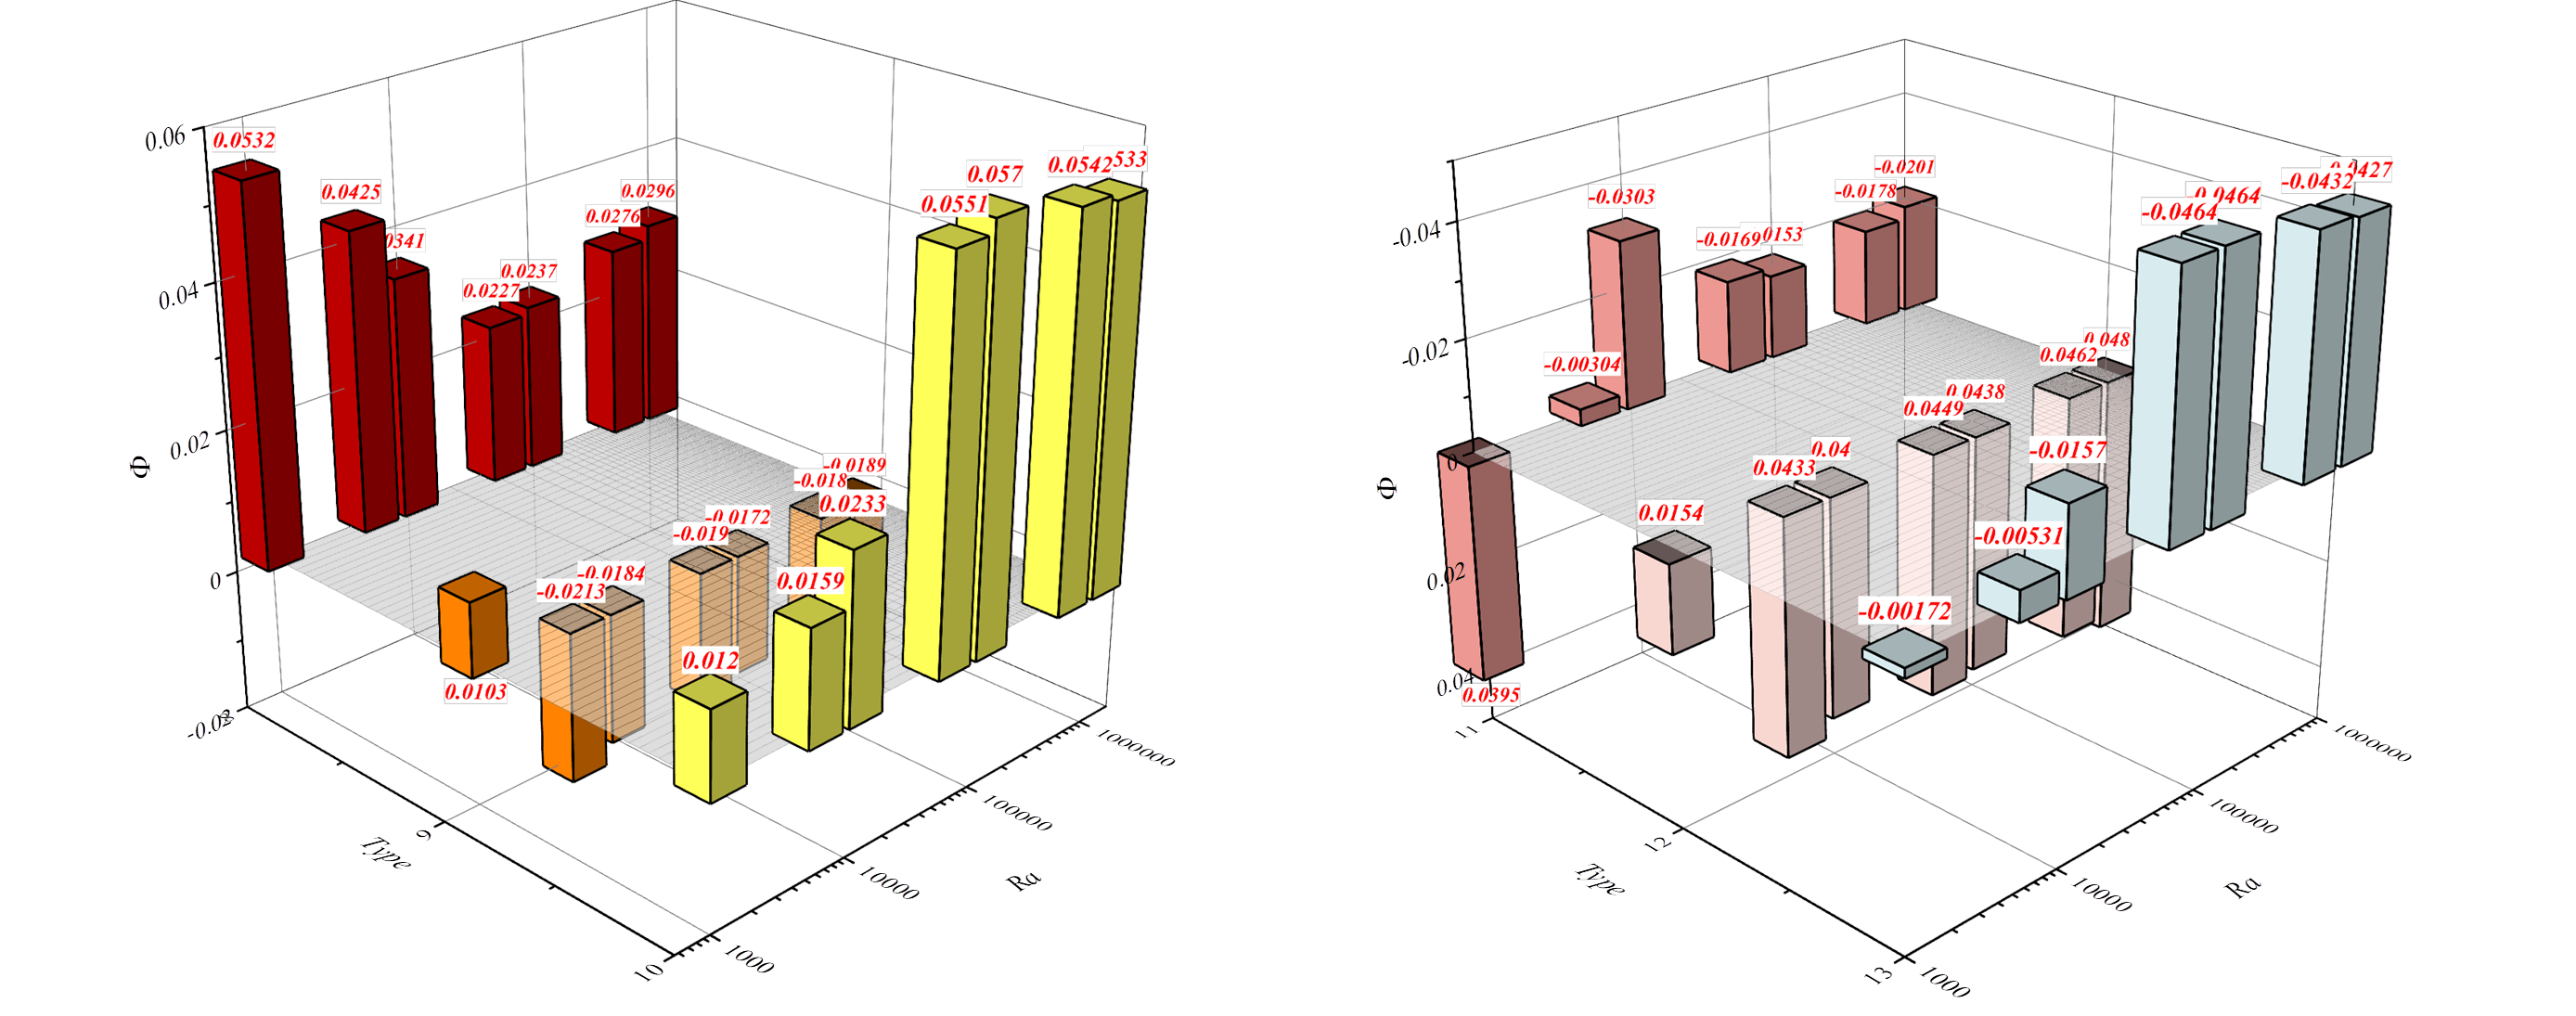
\includegraphics[scale=0.7]{Fig/3d.png}
	\caption{Relative melting time with Rayleigh number  }  
	\label{Fig_Ra} 
\end{figure}
Furthermore, the liquid fractions in the upper left and lower left regions take the lead in the change, and from the conclusions obtained from the analysis in the previous section, convection is stronger on the upper left side than on the lower left side, and therefore it is possible to reduce the volume fraction of the lower left side, which is distributed according to type 10 and type 12, allowing for a faster transfer of heat to the right side. 

Compare and analyse the melting rates of different volume fractions under the same structure based on the conclusions drawn from Fig.\ref{Fig_Ra}. The analysis of Fig.\ref{Fig_3.3fl2} leads to the conclusion that under the same structure, strengthening the volume fraction of the portion known to have intense heat exchange can accelerate the melting rate and a higher heat exchange efficiency can be achieved.
Therefore compare several types of heat transfer that can be intensified.
Until the Rayleigh number is less than $ 5\times10^3 $, the distributions of type 2 is longer than type 8 in relative complete melting time.
At Rayleigh number = $ 5\times10^3 $, the distributions of type 6 is shorter than type 11 in terms of relative complete melting time. 
For the same reason, the distributions of type 7 is shorter than type 13 in terms of relative complete melting time. 
However, they are all shorter than the control group because their values are less than zero. 
In the remaining cases, the distributions of $\Delta\varphi$ = $ 0.02 $ is shorter than $\Delta\varphi$ = $ 0.01 $ in relative complete melting time. Overall the complete melting time for the case of $\Delta\varphi$ = $ 0.02 $ is less than that of $\Delta\varphi$ = $ 0.01 $, which can be achieved by boosting the volume fraction of the Warrior.
\begin{figure}[H]
\centering
	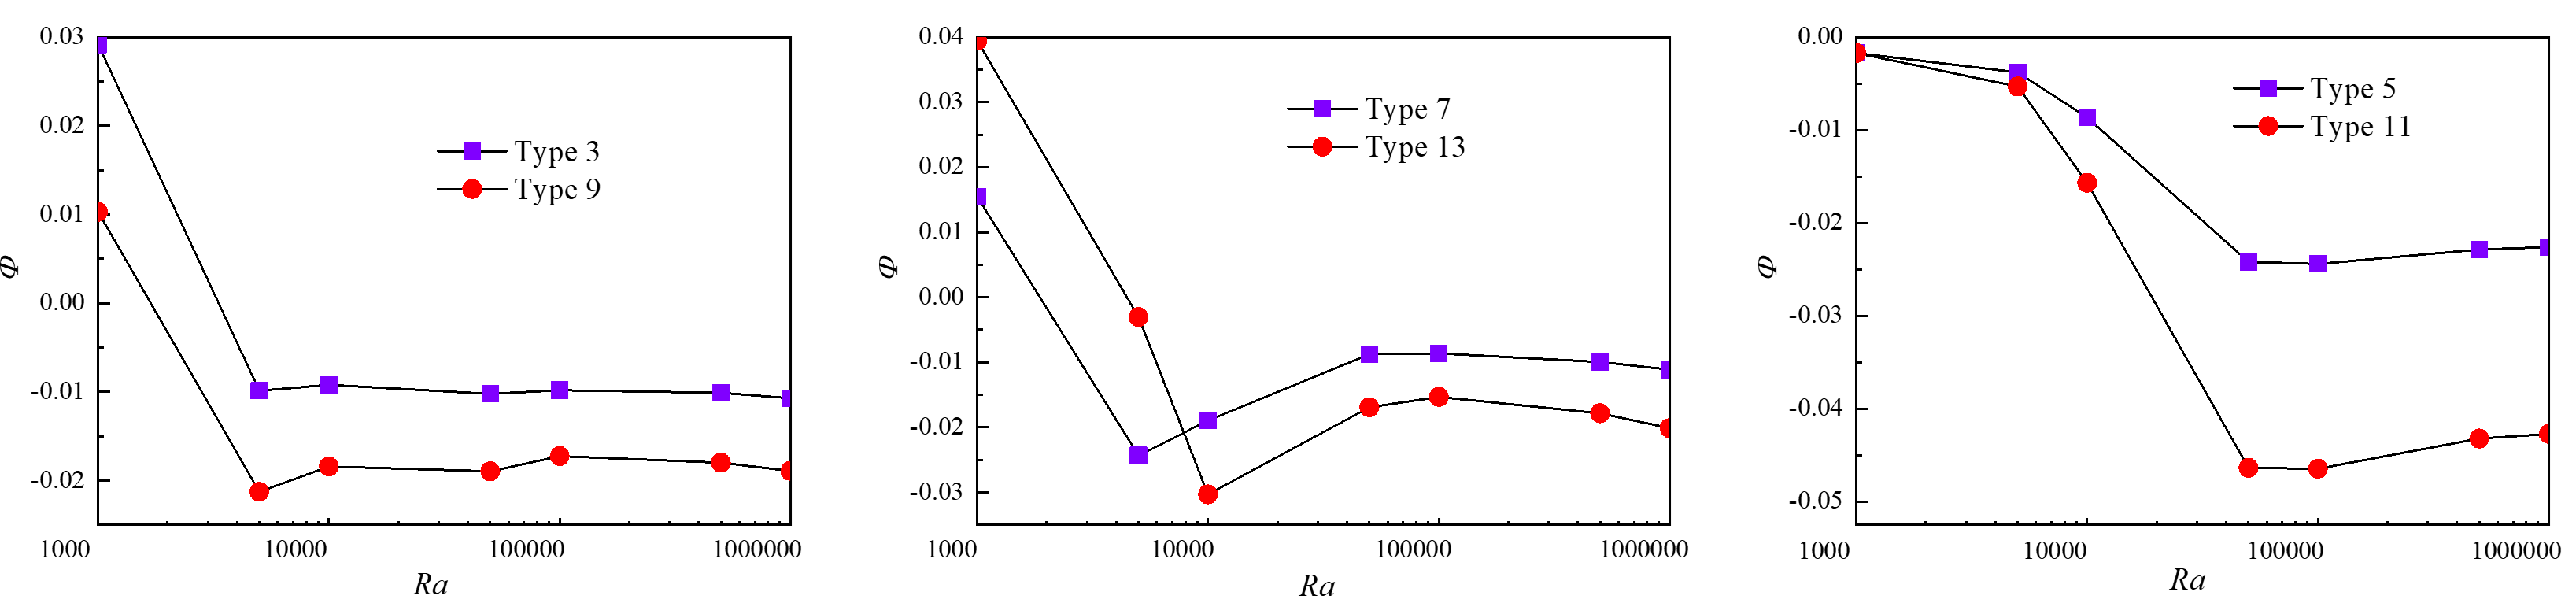
\includegraphics[scale=0.5]{Fig/compare.png}
	\caption{Relative melting time with Rayleigh number  }  
	\label{Fig_3.3fl2} 
\end{figure}

	\section{Conclusions}	

In this paper, a novel TES with optimised NEPCM is proposed. The effects of Rayleigh number, layout pattern and volume fraction on the thermal storage system were investigated by LBM. These analysis can be used to effectively analyse the flow and heat transfer within the heat storage system, and as a result the nanoparticles in the other cavity can be arranged in a reasonable manner. At the same time, the results show that separating the NEPCM by spacers with rational arrangement of spacer arrangement is beneficial to enhance the thermal efficiency of the energy storage system, and the larger the Rayleigh number is, the more drastic the response of the thermal storage system is. The distribution under type 2 has a faster melting rate, which is increased by 2.13\%, 1.84\%, 1.9\%, 1.72\%, 1.8\%, 1.89\% at Rayleigh number change from $ 5\times10^3 $ to $ 10^6 $, compared to that of type 1, respectively. The distribution under type 4 has a faster melting rate with 0.304\%, 3.03\%, 1.69\%, 1.53\%, 1.78\%, 2.01\% increase in melting rate at Rayleigh number change from $ 5\times10^3 $ to $ 10^6 $, compared to type 1. The distribution under type 6 has a faster melting rate, which is enhanced by 0.172\%, 0.531\%, 1.57\%, 4.64\%, 4.64\%, 4.32\%, 4.27\% at Rayleigh numbers$ \geqslant $ $ 10^3 $, respectively, compared to that of type 1. Comprehensive analysis of the upper-left region convection phenomenon is stronger than the lower-left corner, the volume fraction of the right upper and lower regions has little effect on the melting rate, so this heat transfer efficiency can be improved by increasing the volume fraction of the upper-left corner and decreasing the volume fraction of the lower-left corner. And according to the results of this study to produce effective guidance for industrial production. However, the results of this study are based on the spacer material and NEPCM consistent with the basis, need to be under certain special conditions, in the future research process, consider different types of PCM and more arrangement on the heat transfer rate of the impact is also very meaningful.

	\section{Acknowledgements}	
This work was supported by Natural Science Foundation of China (No.52106120).
	
	\bibliographystyle{unsrt}
	
\section{Nomenclature and abbreviations}
The abbreviated and fully qualified forms of the variables covered in this paper are shown in Table \ref{add} and \ref{addd}.

\begin{table}[H]
	\centering
	\footnotesize
	\caption{Individual parameters of Nomenclature}
	\begin{tabular}{cl}
		\toprule
		Nomenclature  &    \\
		\midrule
		\text{c}  & lattice speed[$ m \cdot  s^{-1} $] \\
	$c_{s}$  & lattice sound speed[$ m \cdot  s^{-1} $]    \\
		$C_{p}$ & specific heat at constant pressure[$ KJ \cdot kg^{-1}\cdot K^{-1} $]     \\
	$\boldsymbol{e}_{i}$ & discrete velocity in direction \textit{i}[$ m \cdot  s^{-1} $]  \\
		$F_{i}$ & force[N]    \\
	$f_{i}$& distribution function for density in direction\textit{i}[$ kg \cdot  m^{-3} $]    \\
    $f_i^{eq}$& equilibrium distribution function for density in direction[$ kg \cdot  m^{-3} $]    \\
	$f_{l}$& volume fraction of liquid    \\
	$f_m$&buoyancy force[N]     \\	
	$\mathbf{g}$& acceleration due to gravity [$ m \cdot  s^{-2} $]   \\
    $g_{i}$& distribution function for enthalpy in direction [$ J \cdot  kg^{-1} $]   \\
   	$g_{i}^{eq}$& equilibrium distribution function for enthalpy in direction[$ J \cdot  kg^{-1} $]    \\
	$\text{H}$& the constant height of the fin [m]   \\
	$\text{h}$& total enthalpy [$ J \cdot  kg^{-1} $]   \\
	$\lambda$& thermal conductivity[$ W \cdot m^{-1}\cdot K^{-1} $]      \\
    $\textit{L}$& total length of the heat boundary [m]   \\
   	$\textit{L{s}}$& length of shell cross-section [m]    \\
\textit{$\text{p}$}&  pressure [Pa]   \\	
	\textit{{Q}}& total heat absorption[W]    \\
		\textit{t}& time [s]     \\
$ 	t^{*} $& dimensionless time    \\
	\textit{T}& temperature [K]    \\
$ 	T_{0} $& Initial temperature [K]    \\	
	$ T_{h} $& hot temperature [K]    \\
	$ 	T^{*} $& dimensionless temperature    \\
	\text{u}& velocity [$ m\cdot s^{-1} $]   \\
	\text{x , y}& coordinates [m]   \\
	\textit{$ x^*,y^* $}& dimensionless coordinates    \\
\midrule
Greek symbols  &   \\
\midrule
	$ \alpha $   & thermal diffusivity  [$ m^{2} \cdot  s^{-1} $]   \\
	 $\beta$& thermal expansion coefficient $ 1\cdot K^{-1} $   \\
	 $ \mu $& dynamic viscosity [$ kg\cdot m^{-1}\cdot s^{-1} $]    \\
	 $ \nu $& kinetic viscosity [$ m^{2} \cdot  s^{-1} $] \\
	 $\omega_i$& weight coefficient in direction \textit{i}	\\				
	 $ \varpi _i $& additional weight coefficient in direction   \textit{i}  \\
	$\rho$& density  [$ kg\cdot m^{-3} $]  \\
	$ \tau _f $& dimensionless relaxation time for density distribution function    \\
$ \tau _g $& dimensionless relaxation time for enthalpy distribution function  \\		
	\toprule
	\end{tabular}
\label{add}
\end{table}	\begin{table}[H]
\centering
\footnotesize
\caption{	Subscript and Abbreviation}
\begin{tabular}{cl}
	\toprule
		Subscript   &    \\
		\midrule
PCM  & Pure PCM    \\
bulk & NEPCM   \\
\midrule
Abbreviation   &    \\
\midrule
PCM  & Phase Change Materials    \\
bulk & Nanoparticles enhanced phase change materials   \\
LBM & Lattice Boltzmann Method   \\
TES & Thermal Energy Storage   \\
Ra & Rayleigh number   \\
Ste & Stefan number   \\
Pr & Prandtl Number   \\
	\bottomrule
\end{tabular}
\label{addd}		
\end{table}
	\bibliography{Reference.bib}
\end{document}


